\documentclass{article} % For LaTeX2e
\usepackage{preprint,times}

% Optional math commands from https://github.com/goodfeli/dlbook_notation.
%%%%% NEW MATH DEFINITIONS %%%%%

\usepackage{amsmath,amsfonts,bm}

% Mark sections of captions for referring to divisions of figures
\newcommand{\figleft}{{\em (Left)}}
\newcommand{\figcenter}{{\em (Center)}}
\newcommand{\figright}{{\em (Right)}}
\newcommand{\figtop}{{\em (Top)}}
\newcommand{\figbottom}{{\em (Bottom)}}
\newcommand{\captiona}{{\em (a)}}
\newcommand{\captionb}{{\em (b)}}
\newcommand{\captionc}{{\em (c)}}
\newcommand{\captiond}{{\em (d)}}

% Highlight a newly defined term
\newcommand{\newterm}[1]{{\bf #1}}


% Figure reference, lower-case.
\def\figref#1{figure~\ref{#1}}
% Figure reference, capital. For start of sentence
\def\Figref#1{Figure~\ref{#1}}
\def\twofigref#1#2{figures \ref{#1} and \ref{#2}}
\def\quadfigref#1#2#3#4{figures \ref{#1}, \ref{#2}, \ref{#3} and \ref{#4}}
% Section reference, lower-case.
\def\secref#1{section~\ref{#1}}
% Section reference, capital.
\def\Secref#1{Section~\ref{#1}}
% Reference to two sections.
\def\twosecrefs#1#2{sections \ref{#1} and \ref{#2}}
% Reference to three sections.
\def\secrefs#1#2#3{sections \ref{#1}, \ref{#2} and \ref{#3}}
% Reference to an equation, lower-case.
\def\eqref#1{equation~\ref{#1}}
% Reference to an equation, upper case
\def\Eqref#1{Equation~\ref{#1}}
% A raw reference to an equation---avoid using if possible
\def\plaineqref#1{\ref{#1}}
% Reference to a chapter, lower-case.
\def\chapref#1{chapter~\ref{#1}}
% Reference to an equation, upper case.
\def\Chapref#1{Chapter~\ref{#1}}
% Reference to a range of chapters
\def\rangechapref#1#2{chapters\ref{#1}--\ref{#2}}
% Reference to an algorithm, lower-case.
\def\algref#1{algorithm~\ref{#1}}
% Reference to an algorithm, upper case.
\def\Algref#1{Algorithm~\ref{#1}}
\def\twoalgref#1#2{algorithms \ref{#1} and \ref{#2}}
\def\Twoalgref#1#2{Algorithms \ref{#1} and \ref{#2}}
% Reference to a part, lower case
\def\partref#1{part~\ref{#1}}
% Reference to a part, upper case
\def\Partref#1{Part~\ref{#1}}
\def\twopartref#1#2{parts \ref{#1} and \ref{#2}}

\def\ceil#1{\lceil #1 \rceil}
\def\floor#1{\lfloor #1 \rfloor}
\def\1{\bm{1}}
\newcommand{\train}{\mathcal{D}}
\newcommand{\valid}{\mathcal{D_{\mathrm{valid}}}}
\newcommand{\test}{\mathcal{D_{\mathrm{test}}}}

\def\eps{{\epsilon}}


% Random variables
\def\reta{{\textnormal{$\eta$}}}
\def\ra{{\textnormal{a}}}
\def\rb{{\textnormal{b}}}
\def\rc{{\textnormal{c}}}
\def\rd{{\textnormal{d}}}
\def\re{{\textnormal{e}}}
\def\rf{{\textnormal{f}}}
\def\rg{{\textnormal{g}}}
\def\rh{{\textnormal{h}}}
\def\ri{{\textnormal{i}}}
\def\rj{{\textnormal{j}}}
\def\rk{{\textnormal{k}}}
\def\rl{{\textnormal{l}}}
% rm is already a command, just don't name any random variables m
\def\rn{{\textnormal{n}}}
\def\ro{{\textnormal{o}}}
\def\rp{{\textnormal{p}}}
\def\rq{{\textnormal{q}}}
\def\rr{{\textnormal{r}}}
\def\rs{{\textnormal{s}}}
\def\rt{{\textnormal{t}}}
\def\ru{{\textnormal{u}}}
\def\rv{{\textnormal{v}}}
\def\rw{{\textnormal{w}}}
\def\rx{{\textnormal{x}}}
\def\ry{{\textnormal{y}}}
\def\rz{{\textnormal{z}}}

% Random vectors
\def\rvepsilon{{\mathbf{\epsilon}}}
\def\rvtheta{{\mathbf{\theta}}}
\def\rva{{\mathbf{a}}}
\def\rvb{{\mathbf{b}}}
\def\rvc{{\mathbf{c}}}
\def\rvd{{\mathbf{d}}}
\def\rve{{\mathbf{e}}}
\def\rvf{{\mathbf{f}}}
\def\rvg{{\mathbf{g}}}
\def\rvh{{\mathbf{h}}}
\def\rvu{{\mathbf{i}}}
\def\rvj{{\mathbf{j}}}
\def\rvk{{\mathbf{k}}}
\def\rvl{{\mathbf{l}}}
\def\rvm{{\mathbf{m}}}
\def\rvn{{\mathbf{n}}}
\def\rvo{{\mathbf{o}}}
\def\rvp{{\mathbf{p}}}
\def\rvq{{\mathbf{q}}}
\def\rvr{{\mathbf{r}}}
\def\rvs{{\mathbf{s}}}
\def\rvt{{\mathbf{t}}}
\def\rvu{{\mathbf{u}}}
\def\rvv{{\mathbf{v}}}
\def\rvw{{\mathbf{w}}}
\def\rvx{{\mathbf{x}}}
\def\rvy{{\mathbf{y}}}
\def\rvz{{\mathbf{z}}}

% Elements of random vectors
\def\erva{{\textnormal{a}}}
\def\ervb{{\textnormal{b}}}
\def\ervc{{\textnormal{c}}}
\def\ervd{{\textnormal{d}}}
\def\erve{{\textnormal{e}}}
\def\ervf{{\textnormal{f}}}
\def\ervg{{\textnormal{g}}}
\def\ervh{{\textnormal{h}}}
\def\ervi{{\textnormal{i}}}
\def\ervj{{\textnormal{j}}}
\def\ervk{{\textnormal{k}}}
\def\ervl{{\textnormal{l}}}
\def\ervm{{\textnormal{m}}}
\def\ervn{{\textnormal{n}}}
\def\ervo{{\textnormal{o}}}
\def\ervp{{\textnormal{p}}}
\def\ervq{{\textnormal{q}}}
\def\ervr{{\textnormal{r}}}
\def\ervs{{\textnormal{s}}}
\def\ervt{{\textnormal{t}}}
\def\ervu{{\textnormal{u}}}
\def\ervv{{\textnormal{v}}}
\def\ervw{{\textnormal{w}}}
\def\ervx{{\textnormal{x}}}
\def\ervy{{\textnormal{y}}}
\def\ervz{{\textnormal{z}}}

% Random matrices
\def\rmA{{\mathbf{A}}}
\def\rmB{{\mathbf{B}}}
\def\rmC{{\mathbf{C}}}
\def\rmD{{\mathbf{D}}}
\def\rmE{{\mathbf{E}}}
\def\rmF{{\mathbf{F}}}
\def\rmG{{\mathbf{G}}}
\def\rmH{{\mathbf{H}}}
\def\rmI{{\mathbf{I}}}
\def\rmJ{{\mathbf{J}}}
\def\rmK{{\mathbf{K}}}
\def\rmL{{\mathbf{L}}}
\def\rmM{{\mathbf{M}}}
\def\rmN{{\mathbf{N}}}
\def\rmO{{\mathbf{O}}}
\def\rmP{{\mathbf{P}}}
\def\rmQ{{\mathbf{Q}}}
\def\rmR{{\mathbf{R}}}
\def\rmS{{\mathbf{S}}}
\def\rmT{{\mathbf{T}}}
\def\rmU{{\mathbf{U}}}
\def\rmV{{\mathbf{V}}}
\def\rmW{{\mathbf{W}}}
\def\rmX{{\mathbf{X}}}
\def\rmY{{\mathbf{Y}}}
\def\rmZ{{\mathbf{Z}}}

% Elements of random matrices
\def\ermA{{\textnormal{A}}}
\def\ermB{{\textnormal{B}}}
\def\ermC{{\textnormal{C}}}
\def\ermD{{\textnormal{D}}}
\def\ermE{{\textnormal{E}}}
\def\ermF{{\textnormal{F}}}
\def\ermG{{\textnormal{G}}}
\def\ermH{{\textnormal{H}}}
\def\ermI{{\textnormal{I}}}
\def\ermJ{{\textnormal{J}}}
\def\ermK{{\textnormal{K}}}
\def\ermL{{\textnormal{L}}}
\def\ermM{{\textnormal{M}}}
\def\ermN{{\textnormal{N}}}
\def\ermO{{\textnormal{O}}}
\def\ermP{{\textnormal{P}}}
\def\ermQ{{\textnormal{Q}}}
\def\ermR{{\textnormal{R}}}
\def\ermS{{\textnormal{S}}}
\def\ermT{{\textnormal{T}}}
\def\ermU{{\textnormal{U}}}
\def\ermV{{\textnormal{V}}}
\def\ermW{{\textnormal{W}}}
\def\ermX{{\textnormal{X}}}
\def\ermY{{\textnormal{Y}}}
\def\ermZ{{\textnormal{Z}}}

% Vectors
\def\vzero{{\bm{0}}}
\def\vone{{\bm{1}}}
\def\vmu{{\bm{\mu}}}
\def\vtheta{{\bm{\theta}}}
\def\va{{\bm{a}}}
\def\vb{{\bm{b}}}
\def\vc{{\bm{c}}}
\def\vd{{\bm{d}}}
\def\ve{{\bm{e}}}
\def\vf{{\bm{f}}}
\def\vg{{\bm{g}}}
\def\vh{{\bm{h}}}
\def\vi{{\bm{i}}}
\def\vj{{\bm{j}}}
\def\vk{{\bm{k}}}
\def\vl{{\bm{l}}}
\def\vm{{\bm{m}}}
\def\vn{{\bm{n}}}
\def\vo{{\bm{o}}}
\def\vp{{\bm{p}}}
\def\vq{{\bm{q}}}
\def\vr{{\bm{r}}}
\def\vs{{\bm{s}}}
\def\vt{{\bm{t}}}
\def\vu{{\bm{u}}}
\def\vv{{\bm{v}}}
\def\vw{{\bm{w}}}
\def\vx{{\bm{x}}}
\def\vy{{\bm{y}}}
\def\vz{{\bm{z}}}

% Elements of vectors
\def\evalpha{{\alpha}}
\def\evbeta{{\beta}}
\def\evepsilon{{\epsilon}}
\def\evlambda{{\lambda}}
\def\evomega{{\omega}}
\def\evmu{{\mu}}
\def\evpsi{{\psi}}
\def\evsigma{{\sigma}}
\def\evtheta{{\theta}}
\def\eva{{a}}
\def\evb{{b}}
\def\evc{{c}}
\def\evd{{d}}
\def\eve{{e}}
\def\evf{{f}}
\def\evg{{g}}
\def\evh{{h}}
\def\evi{{i}}
\def\evj{{j}}
\def\evk{{k}}
\def\evl{{l}}
\def\evm{{m}}
\def\evn{{n}}
\def\evo{{o}}
\def\evp{{p}}
\def\evq{{q}}
\def\evr{{r}}
\def\evs{{s}}
\def\evt{{t}}
\def\evu{{u}}
\def\evv{{v}}
\def\evw{{w}}
\def\evx{{x}}
\def\evy{{y}}
\def\evz{{z}}

% Matrix
\def\mA{{\bm{A}}}
\def\mB{{\bm{B}}}
\def\mC{{\bm{C}}}
\def\mD{{\bm{D}}}
\def\mE{{\bm{E}}}
\def\mF{{\bm{F}}}
\def\mG{{\bm{G}}}
\def\mH{{\bm{H}}}
\def\mI{{\bm{I}}}
\def\mJ{{\bm{J}}}
\def\mK{{\bm{K}}}
\def\mL{{\bm{L}}}
\def\mM{{\bm{M}}}
\def\mN{{\bm{N}}}
\def\mO{{\bm{O}}}
\def\mP{{\bm{P}}}
\def\mQ{{\bm{Q}}}
\def\mR{{\bm{R}}}
\def\mS{{\bm{S}}}
\def\mT{{\bm{T}}}
\def\mU{{\bm{U}}}
\def\mV{{\bm{V}}}
\def\mW{{\bm{W}}}
\def\mX{{\bm{X}}}
\def\mY{{\bm{Y}}}
\def\mZ{{\bm{Z}}}
\def\mBeta{{\bm{\beta}}}
\def\mPhi{{\bm{\Phi}}}
\def\mLambda{{\bm{\Lambda}}}
\def\mSigma{{\bm{\Sigma}}}

% Tensor
\DeclareMathAlphabet{\mathsfit}{\encodingdefault}{\sfdefault}{m}{sl}
\SetMathAlphabet{\mathsfit}{bold}{\encodingdefault}{\sfdefault}{bx}{n}
\newcommand{\tens}[1]{\bm{\mathsfit{#1}}}
\def\tA{{\tens{A}}}
\def\tB{{\tens{B}}}
\def\tC{{\tens{C}}}
\def\tD{{\tens{D}}}
\def\tE{{\tens{E}}}
\def\tF{{\tens{F}}}
\def\tG{{\tens{G}}}
\def\tH{{\tens{H}}}
\def\tI{{\tens{I}}}
\def\tJ{{\tens{J}}}
\def\tK{{\tens{K}}}
\def\tL{{\tens{L}}}
\def\tM{{\tens{M}}}
\def\tN{{\tens{N}}}
\def\tO{{\tens{O}}}
\def\tP{{\tens{P}}}
\def\tQ{{\tens{Q}}}
\def\tR{{\tens{R}}}
\def\tS{{\tens{S}}}
\def\tT{{\tens{T}}}
\def\tU{{\tens{U}}}
\def\tV{{\tens{V}}}
\def\tW{{\tens{W}}}
\def\tX{{\tens{X}}}
\def\tY{{\tens{Y}}}
\def\tZ{{\tens{Z}}}


% Graph
\def\gA{{\mathcal{A}}}
\def\gB{{\mathcal{B}}}
\def\gC{{\mathcal{C}}}
\def\gD{{\mathcal{D}}}
\def\gE{{\mathcal{E}}}
\def\gF{{\mathcal{F}}}
\def\gG{{\mathcal{G}}}
\def\gH{{\mathcal{H}}}
\def\gI{{\mathcal{I}}}
\def\gJ{{\mathcal{J}}}
\def\gK{{\mathcal{K}}}
\def\gL{{\mathcal{L}}}
\def\gM{{\mathcal{M}}}
\def\gN{{\mathcal{N}}}
\def\gO{{\mathcal{O}}}
\def\gP{{\mathcal{P}}}
\def\gQ{{\mathcal{Q}}}
\def\gR{{\mathcal{R}}}
\def\gS{{\mathcal{S}}}
\def\gT{{\mathcal{T}}}
\def\gU{{\mathcal{U}}}
\def\gV{{\mathcal{V}}}
\def\gW{{\mathcal{W}}}
\def\gX{{\mathcal{X}}}
\def\gY{{\mathcal{Y}}}
\def\gZ{{\mathcal{Z}}}

% Sets
\def\sA{{\mathbb{A}}}
\def\sB{{\mathbb{B}}}
\def\sC{{\mathbb{C}}}
\def\sD{{\mathbb{D}}}
% Don't use a set called E, because this would be the same as our symbol
% for expectation.
\def\sF{{\mathbb{F}}}
\def\sG{{\mathbb{G}}}
\def\sH{{\mathbb{H}}}
\def\sI{{\mathbb{I}}}
\def\sJ{{\mathbb{J}}}
\def\sK{{\mathbb{K}}}
\def\sL{{\mathbb{L}}}
\def\sM{{\mathbb{M}}}
\def\sN{{\mathbb{N}}}
\def\sO{{\mathbb{O}}}
\def\sP{{\mathbb{P}}}
\def\sQ{{\mathbb{Q}}}
\def\sR{{\mathbb{R}}}
\def\sS{{\mathbb{S}}}
\def\sT{{\mathbb{T}}}
\def\sU{{\mathbb{U}}}
\def\sV{{\mathbb{V}}}
\def\sW{{\mathbb{W}}}
\def\sX{{\mathbb{X}}}
\def\sY{{\mathbb{Y}}}
\def\sZ{{\mathbb{Z}}}

% Entries of a matrix
\def\emLambda{{\Lambda}}
\def\emA{{A}}
\def\emB{{B}}
\def\emC{{C}}
\def\emD{{D}}
\def\emE{{E}}
\def\emF{{F}}
\def\emG{{G}}
\def\emH{{H}}
\def\emI{{I}}
\def\emJ{{J}}
\def\emK{{K}}
\def\emL{{L}}
\def\emM{{M}}
\def\emN{{N}}
\def\emO{{O}}
\def\emP{{P}}
\def\emQ{{Q}}
\def\emR{{R}}
\def\emS{{S}}
\def\emT{{T}}
\def\emU{{U}}
\def\emV{{V}}
\def\emW{{W}}
\def\emX{{X}}
\def\emY{{Y}}
\def\emZ{{Z}}
\def\emSigma{{\Sigma}}

% entries of a tensor
% Same font as tensor, without \bm wrapper
\newcommand{\etens}[1]{\mathsfit{#1}}
\def\etLambda{{\etens{\Lambda}}}
\def\etA{{\etens{A}}}
\def\etB{{\etens{B}}}
\def\etC{{\etens{C}}}
\def\etD{{\etens{D}}}
\def\etE{{\etens{E}}}
\def\etF{{\etens{F}}}
\def\etG{{\etens{G}}}
\def\etH{{\etens{H}}}
\def\etI{{\etens{I}}}
\def\etJ{{\etens{J}}}
\def\etK{{\etens{K}}}
\def\etL{{\etens{L}}}
\def\etM{{\etens{M}}}
\def\etN{{\etens{N}}}
\def\etO{{\etens{O}}}
\def\etP{{\etens{P}}}
\def\etQ{{\etens{Q}}}
\def\etR{{\etens{R}}}
\def\etS{{\etens{S}}}
\def\etT{{\etens{T}}}
\def\etU{{\etens{U}}}
\def\etV{{\etens{V}}}
\def\etW{{\etens{W}}}
\def\etX{{\etens{X}}}
\def\etY{{\etens{Y}}}
\def\etZ{{\etens{Z}}}

% The true underlying data generating distribution
\newcommand{\pdata}{p_{\rm{data}}}
% The empirical distribution defined by the training set
\newcommand{\ptrain}{\hat{p}_{\rm{data}}}
\newcommand{\Ptrain}{\hat{P}_{\rm{data}}}
% The model distribution
\newcommand{\pmodel}{p_{\rm{model}}}
\newcommand{\Pmodel}{P_{\rm{model}}}
\newcommand{\ptildemodel}{\tilde{p}_{\rm{model}}}
% Stochastic autoencoder distributions
\newcommand{\pencode}{p_{\rm{encoder}}}
\newcommand{\pdecode}{p_{\rm{decoder}}}
\newcommand{\precons}{p_{\rm{reconstruct}}}

\newcommand{\laplace}{\mathrm{Laplace}} % Laplace distribution

\newcommand{\E}{\mathbb{E}}
\newcommand{\Ls}{\mathcal{L}}
\newcommand{\R}{\mathbb{R}}
\newcommand{\emp}{\tilde{p}}
\newcommand{\lr}{\alpha}
\newcommand{\reg}{\lambda}
\newcommand{\rect}{\mathrm{rectifier}}
\newcommand{\softmax}{\mathrm{softmax}}
\newcommand{\sigmoid}{\sigma}
\newcommand{\softplus}{\zeta}
\newcommand{\KL}{D_{\mathrm{KL}}}
\newcommand{\Var}{\mathrm{Var}}
\newcommand{\standarderror}{\mathrm{SE}}
\newcommand{\Cov}{\mathrm{Cov}}
% Wolfram Mathworld says $L^2$ is for function spaces and $\ell^2$ is for vectors
% But then they seem to use $L^2$ for vectors throughout the site, and so does
% wikipedia.
\newcommand{\normlzero}{L^0}
\newcommand{\normlone}{L^1}
\newcommand{\normltwo}{L^2}
\newcommand{\normlp}{L^p}
\newcommand{\normmax}{L^\infty}

\newcommand{\parents}{Pa} % See usage in notation.tex. Chosen to match Daphne's book.

\DeclareMathOperator*{\argmax}{arg\,max}
\DeclareMathOperator*{\argmin}{arg\,min}

\DeclareMathOperator{\sign}{sign}
\DeclareMathOperator{\Tr}{Tr}
\let\ab\allowbreak


\usepackage{multirow}
\usepackage{verbatim}
\usepackage{listings}
\lstset{basicstyle=\ttfamily\scriptsize,columns=fullflexible,breaklines=true,breakatwhitespace=false,keepspaces=true,showstringspaces=false,postbreak=\mbox{\ensuremath{\hookrightarrow}\space}}
\usepackage{hyperref}
\usepackage{url}
\usepackage{graphicx}
\usepackage{tikz}
\usepackage{pgfplots}
\pgfplotsset{compat=1.18}

\title{Origami as a Spatial and Geometric Reasoning Benchmark}

\author{Lu Xian \\
LeanMCP \\
\texttt{lu@leanmcp.com}\thanks{Corresponding author: Lu Xian, lu@leanmcp.com.}
\And
Dheeraj Pai \\
LeanMCP \\
\texttt{dheeraj.pai@leanmcp.com}}

% Draft-only appendices (editorial rules, draft status, changes). These are working notes,
% NOT paper content, and must be OFF for any submitted or shared PDF.
% Set \draftnotestrue while drafting; \draftnotesfalse before uploading.
\newif\ifdraftnotes
\draftnotesfalse

\newcommand{\draftimage}[1]{%
  \begin{center}
  \fbox{\parbox[c][#1\baselineskip][c]{0.92\textwidth}{\centering
    \textbf{\footnotesize DRAFT IMAGE: PLACEHOLDER, NOT FINAL}\\[2pt]
    \scriptsize This figure is a draft. It will be replaced with a human-authored
    figure before submission. Drafts are generated with OpenAI \texttt{gpt-image-2}
    via \texttt{paper/figures/gen\_figures.sh} and used only as tracing references;
    no generated image carries data or geometry.\\[6pt]
    \itshape\footnotesize}}
  \end{center}}

\newcommand{\fix}{\marginpar{FIX}}
\newcommand{\new}{\marginpar{NEW}}

\iclrfinalcopy
\begin{document}


\maketitle
\lhead{Preprint}


\begin{abstract}
Many agent tasks require long action sequences whose effects compound and whose result can be
checked only at the end. We introduce \textbf{CP2Seq}, a benchmark for long-horizon sequence planning
with exact verification, built on flat origami. Each of 600 procedurally generated samples gives a
crease pattern and a target folded state, including layer order; the model must find a sequence of
simple folds from an unfolded square. An engine executes or rejects each fold with a named reason,
and a sequence is accepted only if its final stack matches the target layer by layer, including
which region of the sheet each layer comes from. We make no claim about physical folding. We
evaluate GPT-5.6 and GPT-6 Luna under increasing tool assistance and Claude Sonnet 5.5 on 20
instances, counting exact matches with one episode per instance unless stated. The models solve
some short sequences and none of the 20 medium or hard ablation instances (11 or more folds). To
tell whether this reflects the instances or the models, we run random legal folding over the same
actions and budget: it solves 57\% of easy and 96\% of some-layers episodes, while no model
condition solves more than 5 and 8 of the 10 instances. The targets are reachable; the models'
choices are less effective than chance. Their episodes show why. They rarely reach the target and
fail to stop (2 extra solves among 143 logged episodes), they reach a median tenth to a quarter of
the states random folding reaches, and they restart about as often when a repair within three
folds exists as when none does. Support raises totals without removing this pattern: higher
reasoning effort lifts GPT-6 Luna's some-layers solves from 6/30 to 18/30, and legal-fold lists
and target feedback each help. Because the models are given exact coordinates, we also test
whether rendered images add anything; removing them does not lower solve rate, so CP2Seq measures
planning over an exact symbolic state rather than visual perception. Single runs vary
substantially, and depth and layer count are confounded in the deepest group; we report both.
\end{abstract}


\noindent\textbf{Keywords:} origami; spatial reasoning; geometric reasoning; benchmark; multimodal language models; sequential planning

\section{Introduction}
\label{sec:intro}
A locally valid action can lead away from a target. Completing a folding sequence therefore
requires selecting among alternatives, tracking their consequences, and revising earlier
decisions. We study long-horizon planning when the model receives the exact coordinates,
orientations, stacking order and original-sheet regions of every layer, and every action is
checked. Origami provides a generated state space with programmatically checkable success;
we use it as a controlled planning task rather than a model of physical folding.

We introduce \textbf{CP2Seq}: 600 generated instances, a configurable generator, and an
interactive evaluation environment. Given a crease pattern and a target folded state, the
model constructs a sequence of simple folds from an unfolded square. Reference sequences
and intermediate reference states are withheld; any valid sequence producing both the
specified creases and the target stack is accepted. Original-sheet identity and layer order
distinguish geometrically overlapping constructions (Section~\ref{sec:scoring}).

Existing origami benchmarks assess visual questions, pattern prediction or generation
\citep{gamibench,origamispace,origamibench}. CP2Seq instead tests executable sequence
recovery under explicit action constraints. Fold lines are specified in current folded
coordinates while target creases are given on the original sheet; planning connects these
representations through reflections and layer connectivity. Tools expose legality checks,
backtracking, optional legal-action enumeration and target feedback. Search baselines use
the same candidate actions, allowing us to distinguish task reachability from model success.

Our contributions are (1) a generated dataset and generator spanning reference depths and
two simple-fold action models; (2) an interactive pipeline with step-level checks and
replay-based terminal scoring, including original-sheet identity; and (3) matched search
baselines, assistance and modality ablations, repeated trials, and observable trajectory
analysis. These isolate measurable behavior without attributing it to unobserved internal
capabilities.

The models solve some short sequences but no medium or hard ablation instance. Yet random
legal folding solves 57\% of easy and 96\% of some-layers episodes within 80 folds, and BFS
solves five of ten medium instances. Removing images does not reduce solve rate. Failures
rarely reflect reaching the target without stopping; models explore fewer distinct states
than random folding and revisit discarded branches. Repeated trials reveal substantial
variance, while a second model family solves 14/20 instances in one episode each. We
therefore frame CP2Seq as planning over explicit geometric state, not as a validated measure
of visual perception or an isolated internal reasoning faculty. Depth and layer count are
confounded in the released all-layers corpus, limiting depth-based conclusions.

\section{Related work}
\label{sec:related}

\subsection{Origami benchmarks and generation}
\label{sec:related-benchmarks}

GamiBench \citep{gamibench} evaluates multimodal models through visual questions about folded
configurations, viewpoints, and impossible crease patterns. OrigamiSpace \citep{origamispace} evaluates pattern
prediction, multi-step spatial reasoning, spatial relationships, and crease-pattern code generation.
It also provides an interactive environment for the code-generation task, in which the model
writes a crease pattern; CP2Seq instead gives the crease pattern and asks for the fold sequence
that produces it, verified one fold at a time. These benchmarks connect
origami geometry to visual reasoning and generation, with different requirements on the model's
output.

Other recent systems generate origami rather than answer questions about it.
\citet{origamibench} provides an interactive environment for synthesising flat-foldable patterns
over 366
% fact:corpus.instagram.total
designs collected from Flat-Folder, and evaluates query efficiency, defined as the proportion of
fold steps that contribute to the final model, together with geometric and semantic similarity.
Its model adds one crease per step, the environment checks local flat-foldability, and the final
state is scored by image overlap and CLIP similarity to the target; layer order is not verified.
CP2Seq instead asks for a sequence of simple folds and checks the final stack exactly, layer by
layer and by sheet region.
\citet{corigami} pairs a generator with a designer in a pipeline for flat-foldable and visually
recognisable models, using a vision-language model for aesthetic and semantic evaluation and
reporting the flat-foldability of generated crease patterns separately.
\citet{learn2fold} plans structured origami generation against a learned world model.
\citet{foldingagent} works in the opposite direction from generation and the closest to ours: it
reconstructs a folding process from instructional video, using the sequence-level corpus of
\citet{purelandfold}. That corpus is the nearest existing collection to what CP2Seq needs, and we
neither train nor evaluate on it: its sequences are human-authored and its 27 sequences over 337
frames are too few to stratify, whereas ours are generated to order and correct by construction.

\subsection{Computational origami and sequence planning}
\label{sec:related-theory}

A \emph{simple fold} is the operation introduced by \citet{arkin-map} for map folding: the sheet is
folded along one line at a time, by $\pm 180^\circ$. The models are distinguished by how much of the
stack that line carries, namely a single layer, a contiguous run from the top or bottom
(some-layers), or the entire stack (all-layers). A crease pattern is \emph{simply foldable} in a
given model when some sequence of such folds flattens the sheet and leaves exactly its creases.
Deciding that is a studied question whose difficulty depends on the shape of the sheet, the
directions the creases take, and which of the models is permitted
\citep{arkin-map,akitaya-hard}.

CP2Seq uses the some-layers and all-layers variants; the all-layers model is also the one that
describes sheet-metal bending, where it has been studied in its own right
\citep{akitaya-infinite}, and the decision problem has been examined for further restrictions on
the crease directions \citep{mixed-orthogonal}. Work on flat-folded states studies layer ordering
as well as planar geometry \citep{bern-hayes,akitaya-flatfolder,layer-algebra}, motivating our
explicit representation of layers in the state and final comparison; the space of flat foldings
has also been studied as a graph in its own right \citep{flat-folding-graphs}.

A folded state is not a folding motion. Every well-behaved folded state of a simple polygon of
paper is reachable by some continuous motion \citep{continuous}, extending an earlier result for
rectangular paper \citep{reaching-folded}. Those results do not carry over to a restricted
sequence of simple folds; each target here is generated by a recorded legal sequence, so what
makes a sequence hard is not whether the paper can get there but which discrete steps are
permitted along the way. That is the
structure this benchmark measures, and it is why the environment rules on one fold at a time
rather than on a final configuration. Earlier work also addresses generating folding sequences from crease
patterns \citep{akitaya-cp2seq}; sequence recovery is therefore an established computational
origami problem. We use it to evaluate language models as planners over an exact state, with
executable actions, per-step feedback and search baselines on the same instances.

\section{CP2Seq: task and dataset}
\label{sec:cp2seq}

\section{Problem formulation}
\label{sec:problem}

\subsection{Flat-folded states}
\label{sec:problem-states}

A flat-folded state is an isometric map of the sheet into the plane together with a layer
ordering. The map is fixed by the crease pattern; the ordering is not. A single crease pattern
therefore admits many folded states that are geometrically identical and distinct as embeddings,
and determining the ordering is NP hard even when a valid mountain-valley assignment is given
\citep{bern-hayes}.

This distinction is the reason the task cannot be reduced to geometry. Over a folding sequence the
crease graph's topology never changes: the same vertices, edges and faces exist at step one and at
step nineteen. What changes is everything else. Vertex coordinates are reflected at every step.
The overlap structure, which faces lie above which, changes at every step and follows from the
geometry. The layer ordering changes at every step and does \emph{not} follow from the geometry;
it is chosen, and it is where the decisions live. The number of layers accumulates, which is the
formal content of ``it gets harder as it goes''.

\subsection{The action space}
\label{sec:problem-actions}

Simple folds come in named variants, and any benchmark in this area has to say which it uses,
because the complexity results differ between them.

\begin{table}[h]
\caption{Named variants of the simple fold \citep{arkin-map}.}
\label{tab:action-space}
\begin{center}
\begin{tabular}{ll}
\multicolumn{1}{c}{\bf MODEL}  &\multicolumn{1}{c}{\bf DEFINITION} \\
\hline \\
One-layer simple fold    & Rotate a single layer $\pm 180^\circ$ about a line \\
Some-layers simple fold  & Rotate a contiguous run of layers \\
All-layers simple fold   & Rotate every layer the line crosses, as sheet metal bends \\
Finite vs infinite line  & Whether the fold line is a full line or a segment \\
\end{tabular}
\end{center}
\end{table}

CP2Seq instantiates the all-layers and some-layers tiers. The all-layers tier is the simpler
object and it buys three properties at once, the third of which is rarely named. Because the whole
stack moves as a rigid body, no two connected pieces of paper ever move relative to each other
except at the fold line itself, where paper is allowed to bend. Self-intersection is impossible,
the layer ordering is forced rather than chosen, and \textbf{tearing is impossible by
construction.}

Moving only some layers brings all three back, and tearing becomes the binding constraint. If a
moving face is joined to a stationary face along a crease, and that crease is not on the fold
line, the fold would rip the sheet. This is decidable only in the coordinates of the original
square, because adjacency is a fact about the original sheet that survives any amount of folding
and cannot be recovered from the current positions of the polygons alone.

An example makes the tier difference concrete, and it needs only two folds. Fold the right half of
a square over to the left across the vertical midline. The result is a two-layer stack whose top
layer is joined to the bottom layer along the entire crease at the midline. Now select the top
layer alone. Folding its upper half down across the horizontal midline would tear the sheet,
because the moving piece is joined to stationary paper along a vertical crease segment that is
perpendicular to the fold line. Folding its left quarter across a vertical line does not tear,
because the moving piece's only join to stationary paper lies on the fold line itself. Same state,
same layer selection, opposite verdicts, and the only difference is the orientation of the line.

------this 3 paragraphs are over emphasizing on whether all layers fold or some layer'fold  it
gonna tear or not. is that the only point in this part????

\subsection{The task}
\label{sec:problem-task}

Given a crease pattern, produce a sequence of simple folds that reproduces it. Generating an
instance costs one forward pass of the engine; solving it is NP hard. That asymmetry is the
paper's foundation.

---------

It is tempting
to say that legal moves are rare and that this is what makes the task hard. Enumeration refutes
it: legal partial folds \emph{grow} with depth, from 22 at two layers to 332 at thirty-eight, six
times the 56 all-layers folds available at the same state. What falls is the hit rate of uniform
random proposal, from 11.9\% to 3.8\% by seventeen layers, because the space being sampled grows
faster than the legal set inside it. That is a fact about a sampler, not about origami, and
conflating the two would put a false statement about branching factor into the paper.

---------this paragraph should be listed properly and give a proper graph to illustrate it!!!!!!!!



\subsection{Dataset construction}
\label{sec:cp2seq-generation}
\label{sec:cp2seq-why}
\label{sec:cp2seq-difficulty}

Starting from a square sheet, the generator samples a legal fold under the chosen action model,
applies it, and records the action and resulting state. This process continues to the requested
reference depth; attempts with no available legal continuation are discarded. The accumulated
creases are mapped to the original sheet to form the input crease pattern, with edges split at
intersections. The last state supplies the target, and the recorded actions supply a reference
solution. A replay check compares the generated sample with its recorded construction.

We group samples by reference fold count, hypothesizing that longer sequences generally require
more search and are therefore harder to recover. These groups describe expected difficulty;
reference length need not equal the shortest valid solution length. We also record coupling,
the number of creases created by a fold, to characterize the geometry of each instance.

\subsubsection{Generation pseudocode}

{\small\begin{verbatim}
GENERATE(reference_depth, action_model):
    state <- unfolded square
    actions, frames <- [], []
    for step in 1..reference_depth:
        candidates <- LEGAL_FOLDS(state, action_model)
        if candidates is empty: return FAILED
        action <- SAMPLE(candidates)
        state <- APPLY(state, action)
        actions.append(action)
        frames.append(state)
    cp <- CREASE_PATTERN_IN_ORIGINAL_SHEET(state)
    cp <- SPLIT_EDGES_AT_INTERSECTIONS(cp)
    if not REPLAY_CHECK(cp, actions, state): return FAILED
    return (cp, state, actions, frames, METADATA(actions))
\end{verbatim}}

\begin{figure}[t]
\centering
\fbox{\parbox[c][8\baselineskip][c]{0.9\linewidth}{\centering
\textbf{Dataset examples: placeholder}\\[6pt]
Three rows: easy all-layers, deeper all-layers, and some-layers.\\[4pt]
Each row: input crease pattern $\vert$ target folded state $\vert$
reference folding sequence.\\[4pt]
Replace with renders from actual dataset samples.}}
\caption{Planned examples from CP2Seq. Each row will show the two task inputs and the recorded
reference sequence, which is withheld during evaluation. Target views will show both geometry
and layer structure. This placeholder contains no sample data.}
\label{fig:dataset-examples}
\end{figure}

\subsection{Dataset statistics}
\label{sec:dataset-statistics}
\label{sec:cp2seq-contents}

% EDITING NOTE (retained): This part only needs to let readers know that there are
% all-layers folds (easy, medium, hard levels) and some-layers folds.
% EDITING NOTE (retained): Other things like generated or verified can be put in
% Hugging Face or the appendix rather than emphasized here.

CP2Seq contains 600 samples: 400 all-layers examples grouped by reference depth and 200
some-layers examples with three to six reference folds (Table~\ref{tab:dataset-statistics}).
These counts describe distinct dataset samples, not evaluation attempts.

\begin{table}[h]
\centering
\caption{Dataset composition. Fold counts refer to recorded reference sequences.}
\label{tab:dataset-statistics}
\begin{tabular}{llrr}
\hline
Action model & Stratum or group & Samples & Reference folds \\
\hline
All-layers & Easy & 200 & 4--10 \\
All-layers & Medium & 100 & 11--13 \\
All-layers & Hard & 100 & 14--19 \\
Some-layers & Depth 3 & 50 & 3 \\
Some-layers & Depth 4 & 50 & 4 \\
Some-layers & Depth 5 & 50 & 5 \\
Some-layers & Depth 6 & 50 & 6 \\
\hline
Total & & 600 & 3--19 \\
\hline
\end{tabular}
\end{table}

Each sample contains the task inputs, a reference sequence, and metadata
(Table~\ref{tab:sample-files}). The model receives the crease pattern and target state; reference
actions and intermediate reference states are withheld. Tool availability and target feedback are
configured separately from dataset groups (Section~\ref{sec:target-feedback}).

\begin{table}[h]
\centering
\caption{Contents of a CP2Seq sample.}
\label{tab:sample-files}
\label{sec:cp2seq-sample}
\begin{tabular}{lp{0.68\textwidth}}
\hline
File & Contents \\
\hline
\texttt{cp.fold} & Input crease pattern. \\
\texttt{steps.fold} & Folded states after each reference action; only the final state is supplied
as the target. \\
\texttt{seq.json} & Withheld reference actions: fold lines, directions, layer selections, and
creases created. \\
\texttt{meta.json} & Sample descriptors and generator version. \\
\hline
\end{tabular}
\end{table}

\phantomsection
\label{sec:cp2seq-verify}
Reference sequences are checked by replaying them and comparing the resulting creases with the
stored pattern. The two corpus checks reported in this release pass on all 600 samples; they
share the folding engine and therefore do not independently validate its physical assumptions.

\phantomsection
\label{sec:cp2seq-limits}
% EDITING NOTE (retained): "Two limits that belong in the paper rather than an appendix -- MISSING."
% The two issues are limited coverage of long sequences with low coupling, and
% the six-fold maximum reference depth of the some-layers subset.
Coverage is limited in two respects: long reference sequences with low coupling are sparsely
represented by the generation procedure, and some-layers examples extend only to six reference
folds. These are limits of the present corpus, not proofs that other configurations are impossible.

% FIGURE NOTE (retained): Plot fold depth against coupling, shaded by sample count.
% Check the actual counts before describing a cell as empty; the earlier draft
% reported two hits in 16,000 attempts, which does not establish impossibility.
% The draft difficulty-grid placeholder has been removed from the main text.

\section{Experimental setup}
\label{sec:experimental-setup}
\subsection{Environment}
\label{sec:env}
\label{sec:env-one-object}
\label{sec:env-division}

The model edits a folding sequence through the tools in Table~\ref{tab:tools}. For each proposed
fold, the engine reflects the selected paper across the fold line, updates layer order and
orientation, and checks sheet connectivity and compatibility with the input crease pattern.
Accepted edits update the current state; rejected edits return an error code and preserve the
previous state.

\phantomsection
\label{sec:env-refusals}
% EDITING NOTE (retained): Explain checks for each step and the final state.
For a some-layers fold, moving and stationary regions may share an edge away from the hinge.
Reflecting only the moving region would separate that shared edge, so the engine rejects the
proposal as \texttt{would-tear}. A \texttt{no-crease} rejection means that paper was selected to
move but the operation did not create a crease segment. Other rejections cover an empty moving region, an incompatible over/under direction,
and creases absent from the target pattern. That last check is a form of assistance: it prevents a
class of unrecoverable moves, and the rates reported here are therefore rates under that
constraint. Detailed conditions are listed in
Appendix~\ref{app:action-errors}.

The environment restricts moving layers to the whole stack or a contiguous top/bottom run.
It checks flat endpoint states and connectivity, but does not verify continuous collision-free
motion; endpoint legality is therefore not a physical realizability guarantee.

\phantomsection
\label{sec:env-observes}
% EDITING NOTE (retained): Add a screenshot of the simulator interface.
Observation tools are listed in Table~\ref{tab:tools}. Exploded views use illustrative
layer separation.

\subsection{Evaluation metrics}
\label{sec:scoring}

\phantomsection
\label{sec:scoring-why}
We accept any executable sequence that produces the required crease pattern and folded state.

\subsubsection{Verification}
\label{sec:scoring-what}

We execute the proposed sequence and compare its accumulated creases with the input pattern,
including mountain--valley assignments. We then compare the final stack with the target after
alignment by a single global translation, rotation, or turnover. A turnover reflects the geometry,
reverses the stack order, and flips face orientations. The same transformation must align all
layers in their corresponding stack order.
A successful construction must satisfy both crease-pattern and folded-state agreement.

\paragraph{Equivalence relation.} The submitted results used plane equivalence
($E_{\mathrm{plane}}$): one isometry carries every layer polygon and parity onto the target's at
the same rank. The task definition also requires each rank to hold the same region of the
original sheet, up to a symmetry of the crease pattern ($E_{\mathrm{id}}$,
Appendix~\ref{app:comparison-details}). Two stacks equal in the plane but interleaving the sheet
differently are different objects. We now score with $E_{\mathrm{id}}$, report both, and count
$E_{\mathrm{plane}}$-only solves as unsolved (Appendix~\ref{app:identity-audit}).

\paragraph{Audit and scope.}
Crease-pattern agreement does not remove identity ambiguity. In the reported audit of
536 previously accepted episodes, 514 pass $E_{\mathrm{id}}$; the 22 reversals include
18 model and four BFS solutions. The primary 360-case ablation total changes from
55 to 50 solves (Table~\ref{tab:luna-ablations}). Identity-sensitive regression tests
include congruent layers with permuted sheet regions; these pass the plane test but
must fail the identity test (Appendices~\ref{app:comparison-details}
and~\ref{app:identity-audit}). These corrections concern terminal outcomes, separately
from defects in feedback shown during search.

The crease comparator and the shared folded-state
comparator both match positions within $2\times10^{-6}$; Table~\ref{tab:tolerances} lists every
tolerance in the pipeline, and Appendix~\ref{app:comparison-details} describes the alignment and
representation details.

\subsubsection{Reported metrics}
\label{sec:scoring-metrics}

We report solve rate by fold-count group, with the number of attempts and the applicable run
budgets. Termination reasons distinguish successful submission, unsuccessful completion, budget
limits, and repetition-related stopping. Query counts measure calls consumed before termination.

% EDITING NOTE: Compute CP edit distance for the final valid state of every saved attempt,
% including unsuccessful and interrupted runs. Define edits, costs, normalization, and treatment
% of missing state artifacts before adding numerical results. See IMPORTANT_TODO.md.
We measure CP edit distance between the accumulated crease pattern in the last recoverable
state and the supplied pattern, in original-sheet coordinates. Collinear mountain and valley
intervals are merged separately, excluding sheet boundaries. If $m$ intervals match under the
crease comparator, the insertion/deletion distance is
$d_{\mathrm{CP}}=|C_{\mathrm{target}}|+|C_{\mathrm{candidate}}|-2m$.
Each missing or extra interval costs one; changing an assignment costs two. Partially overlapping
intervals do not match unless their endpoints agree within tolerance. We also report
$d_{\mathrm{CP}}/|C_{\mathrm{target}}|$, which can exceed one. Normalized distance is undefined
for an empty target. Means weight attempts equally and exclude missing state artifacts,
whose counts are reported separately.

\phantomsection
\label{sec:scoring-validate}
Verification is operational and tolerance-based, not a formal proof in exact arithmetic.
Comparator implementation and validation cases are described in
Appendix~\ref{app:comparison-details}.

\subsection{Evaluation protocol}
\label{sec:experiments}

The Luna interface uses OpenAI Codex CLI \citep{openai-codex} through a custom
episode harness; the added Sonnet experiments use Claude Code CLI with the same task tools. Software version evidence is documented in
Appendix~\ref{app:software-versions}.

% EDITING NOTE (retained): The pipeline -----should have a hand drawn graph
\subsubsection{Episode procedure}
\label{sec:exp-pipeline}

One episode is one sample attempted by one model under one tier of assistance. The loop is the same
for every arm and every model, and the only thing that varies between arms is what the model is
allowed to see and call.

Each query contains one tool call. Accepted edits update the current sequence;
rejected edits preserve it, and both consume budget. Removing a fold replays the remaining actions;
returning to an earlier step truncates the sequence, while revision restoration can recover a
previous branch. The reference sequence is withheld until scoring.

% ===========================================================================
% FIGURE 4 -- THE EVALUATION PIPELINE.  [TO DRAW]
% Left-to-right diagram of one episode.
%   LEFT    the two inputs: crease pattern, final folded state.
%   CENTRE  the loop as a cycle: model proposes a fold; environment returns either
%           a new state with its two rendered views, or a NAMED refusal; history
%           accumulates.
%   RIGHT   termination and scoring: replay of the model's sequence and replay of
%           the reference, compared at Level 1 and Level 2.
% Must make three things visually obvious:
%   (1) environment and verifier are ONE box, not two;
%   (2) refusals loop back WITHOUT advancing;
%   (3) seq.json sits OUTSIDE the loop, entering only at scoring.
% A dashed boundary around the withheld items (intermediate frames, reference
% sequence) carries point (3) without a sentence.
% ===========================================================================
Episode pseudocode and the evaluation pipeline appear in
Appendix~\ref{app:evaluation-pipeline}.

\phantomsection\label{sec:exp-tools}
All conditions provide fold editing, backtracking, and state observations. Additional
conditions provide legal-fold enumeration and target feedback
(Section~\ref{sec:ablations}). The full tool interface and loading configuration
appear in Appendix~\ref{app:tool-interface}.

% ===========================================================================
% FIGURE 5 -- A REFUSAL AS THE MODEL RECEIVES IT.  [TO DRAW]
% One concrete rejected fold, rendered exactly as the harness returns it:
%   - the proposed fold line drawn over the current state;
%   - the named reason (would-tear);
%   - the specific evidence: for a tear, the crease segment joining a moving face
%     to a stationary one, highlighted, away from the fold line.
% Beside it, the SAME state with a legal fold line, for contrast. This is the
% tearing pair of the action-space section, which currently exists only as prose.
% Caption states that the reason is a NAME rather than a boolean, and that this is
% why error analysis is a taxonomy that exists before the experiment.
% ===========================================================================
% EDITING NOTE: Refusal figure moved to the appendix plan; use an actual rejected action.

\subsubsection{Models and budgets}
\label{sec:exp-protocol}

The recent ablations evaluate GPT-5.6 Luna at low reasoning effort and GPT-6 Luna
at low and high effort, using ten samples per group and configuration. Runs use an
80-turn limit, a 300-second call timeout, and full image history. Earlier runs have
different coverage and budgets and are reported separately (Section~\ref{sec:results}).
% EDITING NOTE: Report per-run stopping limits and repeat variability from the inventory.

We include breadth-first search over the same enumerated legal actions as a
systematic-search baseline (Appendix~\ref{app:bfs-analysis}).
% EDITING NOTE: Planned baselines retained for future work: uniform random search
% over legal candidates and the symbolic crease-pattern solver cited as creasy.

\subsection{Assistance conditions}
\label{sec:ablations}

% EDITING NOTE: Planned comparisons retained: no visual feedback and verifier only.
The ablations compare tool conditions with common sample IDs and budgets: \emph{basic tools}
(B; the interface of Section~\ref{sec:exp-tools}), \emph{legal enumeration} (L; B plus
\texttt{list\_legal\_folds}), and \emph{legal enumeration with automatic feedback} (L+A; L plus
tier-3 target feedback after every accepted edit). A fourth condition, B+A, gives automatic
feedback without legal enumeration, so that the two additions can be measured separately
(Section~\ref{sec:results-feedback-only}). Earlier runs instead let the model request tier-3
comparison on demand.
\phantomsection\label{tab:ablations}

\phantomsection
\label{sec:target-feedback}
Automatic feedback supplies layer counts, aligned layer discrepancies,
and suggested corrections after edits (Appendix~\ref{app:feedback-levels}). Because those
corrections do much of the target comparison for the model, we treat the feedback conditions as an upper
bound on what tool support can achieve with this model, not as a measure of the model's own geometric reasoning;
conclusions about the model rest on the basic-tools condition. Even that condition is assisted,
since folds that would crease outside the target pattern are rejected (Section~\ref{sec:env}).

\section{Results}
\label{sec:results}

We report the completed Codex runs in the inventory generated on 24 September 2026,
separating the broader GPT-5.6 Luna evaluation from the recent ablations. The inventory
counts completed attempts, including unsuccessful submissions and stopping-limit
terminations. For the ablations, all 360 planned sample--configuration pairs enter
the denominator. Execution errors and omissions after blocking errors count as
unsuccessful evaluations, with causes marked separately. We retain the first completed
attempt per sample and configuration when available; retries do not add denominator entries.
% Source: workspace/RESULTS/run-inventory/report.md (2026-09-24T23:13:33.275Z).
% Generated with workspace/report_run_inventory.mjs; per-attempt provenance is in report.json.
% The prior Results section and its editorial notes are preserved in
% sections/09-results-previous-snapshot.tex, but are not included in the paper.

\phantomsection\label{sec:results-headline}
Earlier GPT-5.6 Luna runs used different samples and budgets per condition, so we list them
without comparison (Table~\ref{tab:headline}); tool effects are measured only in the ablations.

\subsection{Tool and reasoning-effort ablations}
\label{sec:results-tiers}
\label{sec:results-ablations}

The recent study uses the first ten samples of each group in every configuration:
\texttt{easy-}, \texttt{mid-} and \texttt{hard-0001}--\texttt{0010} from the all-layers corpus and
\texttt{layers-0001}--\texttt{0010} from the some-layers corpus; the some-layers samples all have five reference folds. It compares GPT-5.6 Luna at low effort with
GPT-6 Luna at low and high effort. Tool conditions and run settings are
given in Sections~\ref{sec:ablations} and~\ref{sec:exp-protocol}. Of the 360 planned
sample--configuration pairs, five are protocol failures counted as unsolved
(Appendix~\ref{app:protocol-failures}).

\paragraph{Sample selection.} IDs follow consecutive generator seeds and were fixed before any
ablation run; the selected samples match their groups in depth but have somewhat fewer layers and
creases, so their solve rates if anything overstate the full groups' (Appendix~\ref{app:sample-selection}).

\begin{table}[htbp]
\centering
\caption{Recent Luna ablations. Cells show solved/evaluated samples; each group
has ten intended samples. B: basic tools; L: legal enumeration; A: legal enumeration
with automatic tier-3 target feedback. $*$ includes one input-size error;
$\dagger$ includes one service prompt rejection; $\ddagger$ includes two
omissions after blocking errors. All five count as unsuccessful evaluations. In two A cells
(easy, GPT-5.6 low and GPT-6 high) one wrong submission followed a false \emph{matches} from the
comparison tool (Appendix~\ref{app:protocol-failures}). Counts are under the identity-aware
relation $E_{\mathrm{id}}$ (Section~\ref{sec:scoring-what}); \pending{k} cells change from the
submitted $E_{\mathrm{plane}}$ counts, which are listed in Appendix~\ref{app:identity-audit}.}
\label{tab:luna-ablations}
\small
\setlength{\tabcolsep}{4pt}
\begin{tabular}{lllrrrrr}
\hline
Model & Effort & Tools & Easy & Medium & Hard & Some-layers & Total \\
\hline
GPT-5.6 Luna & Low & B & 2/10 & 0/10 & 0/10 & 0/10 & 2/40 \\
 & Low & L & 1/10 & 0/10 & 0/10 & 5/10 & 6/40 \\
 & Low & A & 4/10 & $0/10^{*}$ & 0/10 & 6/10 & $10/40^{*}$ \\
\hline
GPT-6 Luna & Low & B & 0/10 & 0/10 & 0/10 & 0/10 & 0/40 \\
 & Low & L & 1/10 & $0/10^{*\dagger}$ & 0/10 & 1/10 & $2/40^{*\dagger}$ \\
 & Low & A & 3/10 & $0/10^{\ddagger}$ & 0/10 & 5/10 & $8/40^{\ddagger}$ \\
\hline
GPT-6 Luna & High & B & 3/10 & 0/10 & 0/10 & 3/10 & 6/40 \\
 & High & L & 3/10 & 0/10 & 0/10 & 7/10 & 10/40 \\
 & High & A & 3/10 & 0/10 & 0/10 & 8/10 & 11/40 \\
\hline
\end{tabular}
\end{table}

\paragraph{Tools.} Summing the Total column of Table~\ref{tab:luna-ablations} over the three model
settings gives, for the same 40 samples in each, 8/120 solves with B, 18/120 with L and 29/120
with A (two L and three A pairs are protocol failures counted as unsolved); the order B$<$L$<$A
holds in each setting. By group, easy gives 5, 5 and 10 of 30 and some-layers 3, 13 and 19 of 30;
medium and hard give none. Clustering by instance, the pooled differences are
\pending{L$-$B} (95\% CI \pending{CI}) and \pending{A$-$L} (95\% CI \pending{CI}); per-cell
comparisons are not individually reliable at ten samples.

\paragraph{Reasoning effort.} Pooled over the three tool conditions, GPT-6 Luna solves 6/30
some-layers samples at low effort and 18/30 at high effort. Per condition the increases are
0/10 to 3/10, 1/10 to 7/10 and 5/10 to 8/10; with ten samples per cell only the second is
significant on its own (two-sided Fisher exact test, $p\approx0.02$; $p\approx0.21$ and $0.35$
for the others), and a 95\% Wilson interval spans roughly $\pm0.3$ (e.g.\ 0.11--0.60 for
3/10). Pairing outcomes by sample and condition, every discordant pair favours high effort
(12 to 0; exact McNemar test, $p<0.001$), so the effect is consistent even where single cells
are underpowered. McNemar treats the 30 sample--condition pairs as independent, but each
some-layers instance appears in all three tool conditions. Treating the instance as the unit,
a cluster bootstrap over the ten instances gives a high-minus-low difference of
\pending{diff} in some-layers solve rate (95\% CI \pending{a} to \pending{b}), and an exact
sign-flip test over per-instance differences gives $p=\pending{p}$; over all 40 instances the
difference is \pending{d} (95\% CI \pending{a'} to \pending{b'}). With ten instances the
interval is wide; the direction is consistent, the size is not well determined. It is measured on five-fold some-layers samples; on the easy group, which spans
four to ten folds, solves rise less, from 4/30 to 9/30.

\paragraph{Depth.} No Luna ablation solves a medium or hard sample, and the breadth-first
baseline solves 1/40 medium and 0/16 hard attempts (Appendix~\ref{app:bfs-analysis}), against
366/669 on the easy group. Within the easy group, the model solve rate falls from 32\% at four folds to
0--15\% at eight to ten (Table~\ref{tab:easy-depth}). The groups differ in more than depth: the
medium and hard samples also have several times more layers and creases (Section~\ref{sec:results-ablations}),
so these results show that the deeper groups are harder, not that depth alone is the cause.
Breadth-first search time on the saved searches grows by a fitted factor of 3.9 per fold on easy
and 4.6 on medium (Figure~\ref{fig:depth-wall}); the hard-group factor of 12.4 rests on two samples
and an extrapolation, and we do not use it as a measure of task complexity.

\subsection{Matched baselines and input modality}
\label{sec:results-matched}

The BFS figures above come from 725 attempts with repeated samples and varying budgets. We
therefore ran a random-legal baseline (100 episodes of 80 folds per instance) and BFS (budgets of
80 to $10^5$ expansions) on exactly the 40 ablation instances, with the models' action space,
enumerator and success criterion (Appendix~\ref{app:matched-trajectories}, Table~\ref{tab:matched}).
\pending{One-sentence summary of Table~\ref{tab:matched}: where the best Luna configuration sits between random-legal and BFS.}


\phantomsection\label{sec:results-textonly}
\paragraph{Text-only input.} To measure what the images contribute, we reran the GPT-5.6 Luna
(low effort) ablation with every image removed from the prompt and from tool results, keeping
the JSON geometry of the crease pattern, target and current state. Under the submitted
$E_{\mathrm{plane}}$ scoring, text-only solves 3, 7 and 11 of 40 with B, L and A, against 2, 6
and 10 with images (pooled 21/120 vs.\ 18/120; discordant pairs 9 vs.\ 6, exact McNemar
$p=0.61$). Two text-only L solves fail $E_{\mathrm{id}}$ (Appendix~\ref{app:identity-audit}), giving
\pending{3, 5, 11} under $E_{\mathrm{id}}$. Either way, removing images does not reduce solve
rate on these samples: the model's successful reasoning runs through the coordinate
description, and the rendered views add no measurable benefit at this sample size. One text-only
basic and two text-only medium episodes ended in protocol failures and count as unsolved.

\subsection{Failure analysis}
\label{sec:results-failures}

Termination labels name the stopping rule that fired, not the cause of failure. Rejected
actions never end an episode, although they consume turns; the cycling rule stops an episode
when the same fold is played from the same position three times. In the ablations, 191 of 300
unsuccessful episodes end under the cycling rule (Table~\ref{tab:ablation-terminations}); in the
earlier 447-attempt GPT-5.6 Luna snapshot, 215 of 384 do. These counts describe how episodes
stopped. To ask why, we analysed every turn of every ablation episode
(Table~\ref{tab:trajectories}), replaying each accepted state and comparing it with the target.

Each unsuccessful episode is assigned one of four mechanical categories
(Appendix~\ref{app:matched-trajectories}): F1, mostly geometrically illegal proposals; F2, mostly
legal folds off the target pattern; F3, the full pattern at the target depth but a wrong stack;
F4, never reaching the target depth. They locate where an episode broke down, not which internal
capability failed.


The completed text-only GPT-5.6 Luna episodes (39 per arm), analysed the same way, show the
pattern the categories are meant to expose. With basic tools, 82\% of proposed folds are rejected,
mostly as off-pattern, and 29 of 36 failures are F2; with legal enumeration, the rejection rate
falls to 13\% and failures shift to F4 (21 of 32) and F3 (6 of 32). Once the tool removes
illegal and off-pattern moves, the remaining failures are episodes that never reach the target
depth, or reach it with the layers in the wrong order.
\pending{Replace with the image-condition ablation numbers once Table~\ref{tab:trajectories} is filled.}

\paragraph{Cycling limit.} Rerunning GPT-6 Luna (high, A) with a limit of six repeats instead
of three turns \pending{c} of its \pending{28} cycling stops into solves (Appendix~\ref{app:matched-trajectories}).

\phantomsection
\label{sec:results-difficulty}
\phantomsection
\label{sec:results-threats}
The broader evaluation, ablations, BFS snapshot and CP-distance scan cover different attempt
sets with different budgets; we report their denominators separately and do not pool them into
a single controlled comparison. The matched comparison of model and search is
Table~\ref{tab:matched}.

\section{Limitations}
\label{sec:limitations}

The evaluation covers Luna models and BFS, and the ablations use ten samples per group and
configuration. This study is currently privately funded, and these limits follow from the cost of
evaluation: with full image history, one Luna episode consumed about 3.1 million input tokens on
average over 20 episodes. In pilots, Qwen3.5-9B (via Tinker) cycled without solving either of two samples, and one
80-turn GPT-6 Astra episode cost about US\$400. We are seeking research funding to extend the evaluation to further
model families and to the full corpus.

The action space covers all-layers and selected some-layers simple folds, excluding
pre-creasing; the some-layers corpus currently extends to six reference folds. The environment
represents zero-thickness flat states and does not model material mechanics or continuous
collisions during folding.

Termination labels record stopping conditions. The trajectory categories of
Section~\ref{sec:results-failures} locate where an episode broke down, but they are mechanical
rules over observable states and do not identify which internal capability failed. Revisit and
budget limits constrain the observed search, and the effect of a looser cycling limit is untested.
Per-turn logs of the image ablations were not retained, so the trajectory analysis covers the
text-only runs only, and the comparison-tool defect cannot be audited call by call there.
Training overlap with the public corpus is unknown.

Corpus replay checks assess consistency with the shared generation engine. The submitted results
were scored with a plane-only terminal comparator that did not check original-sheet region
identity; the identity audit (Appendix~\ref{app:identity-audit}) found accepted solutions that
fail the identity-aware relation, and all results are now re-scored under it. The comparison
tool shown to models still uses the plane-only relation, so its \emph{matches} can be wrong in
the same way; the affected calls are counted in Appendix~\ref{app:protocol-failures}.

\section{Conclusion and future work}
\label{sec:conclusion}

CP2Seq pairs 600 generated instances and an open-ended generator with an environment that rules on
each fold and a scorer that accepts any valid sequence. The experiments support three observations. First, difficulty rises steeply with sequence
depth: models solve some easy and some-layers samples, but no ablation configuration solves a
medium or hard sample, and breadth-first search over the same actions solves 366/669 easy
attempts but only 1/40 medium and 0/16 hard, consistent with a search cost that rises steeply on the deeper groups, which
also have many more layers and creases. On the 40 ablation instances, however, 80 random legal folds per episode solve
57\% of easy and 96\% of some-layers episodes, above the model's per-instance rate, and on medium,
where no model episode succeeds, random folding (3 of 10 instances over 100 episodes each) and
breadth-first search (5 of 10 within $10^5$ expansions) do. The medium group therefore marks a limit
of these models rather than of search; only the hard group is unsolved by every method. Second, in the text-only runs whose turns we could analyse, once legal-fold enumeration removes
illegal and off-pattern moves, unsuccessful episodes mostly never reach the target depth, and some
reach it with the layers in the wrong order; across the ablations most stop under the cycling
rule, which describes how they ended rather than why. Failures are almost never missed stops
(an automatic stop would add 2 solves to 25 in 143 episodes), and models reach a tenth to a
quarter of the distinct states that random folding reaches, which points to exploration as the
bottleneck. Third, assistance and reasoning effort
help within reach but do not move that reach: on matched samples, target feedback and higher
effort raise solve rates on short sequences (target feedback alone and legal-fold enumeration alone
each raise GPT-5.6 Luna from 2/40 to 5/40, and together to 9/40), while medium and hard samples stay
unsolved in every model condition. Because each ablation result rests on ten samples per cell, we report these as trends with
their uncertainty rather than as rankings of models.

Because the generator produces fresh instances with exact, programmatically checkable success,
CP2Seq can also serve as an environment for training rather than only testing, a use we have
not yet evaluated. Next steps are to extend the evaluation to other model families and to the full corpus; to add
a symbolic solver such as \citet{creasy}; and to probe model reasoning directly, so that
failures can be attributed to state tracking, target comparison or backtracking rather than
located by observable state alone. A natural extension is to check generated sequences
with a bar-and-hinge simulator that models contact \citep{swomps}, connecting the benchmark to
engineering folding problems.
\phantomsection\label{sec:main-text-end}

\ifdraftnotes
\section{Figures}
\label{sec:figures}

\begin{table}[h]
\caption{Planned figures and their status.}
\label{tab:figures}
\begin{center}
\begin{tabular}{lp{0.62\textwidth}l}
\multicolumn{1}{c}{\bf \#}  &\multicolumn{1}{c}{\bf FIGURE}  &\multicolumn{1}{c}{\bf STATUS} \\
\hline \\
1 & Task schematic: inputs, sequence construction, and replay checks
    (Figure~\ref{fig:sample}) & Included \\
2 & Optional connectivity example for Appendix~\ref{app:tearing}; verify both actions
    with the engine before drawing & To verify \\
3 & A refusal as the model receives it: view, named reason, per-constraint checklist with
    locations & To draw \\
4 & The difficulty grid, depth against coupling, with the empty cell visible & To draw \\
5 & Main result per group & \texttt{[TO RUN]} \\
\end{tabular}
\end{center}
\end{table}

\fi
\section*{Reproducibility statement}
\label{sec:licence}
\label{sec:reproducibility}
\providecommand{\artifactavailability}{with links omitted for anonymous review}

The task, action models and state representation are specified in Section~\ref{sec:problem} and
Appendix~\ref{app:folding-model}; the generation procedure in Section~\ref{sec:cp2seq-generation}
and Appendix~\ref{app:generation-procedure}; the scoring rule, comparator and every numerical
tolerance in Section~\ref{sec:scoring} and Appendix~\ref{app:comparison-details}; the episode
loop, tool interface, tool schemas and prompt in Appendices~\ref{app:evaluation-pipeline}
and~\ref{app:tool-interface}; model versions, reasoning effort, turn and timeout limits in
Section~\ref{sec:exp-protocol}; the software version in Appendix~\ref{app:software-versions};
and the accounting of every planned ablation case, including failures, in
Appendix~\ref{app:protocol-failures}. The evaluated models are closed and served through the
Codex CLI (Luna) or Claude Code CLI (Sonnet), so their weights and sampling cannot be pinned; we release the saved runs with each
attempt's model identifier and reasoning effort, so reported numbers can be audited if not
regenerated exactly. The corpus generator, environment and verifier, corpus
checks, state comparator and evaluation harness are released under the BSD 3-Clause licence,
\artifactavailability. Every sample is synthesised by folding a square, so the
data carry no personal, human-subject or scraped content; Flat-Folder's example collection is
neither used nor redistributed.

\section*{Use of large language models}
\label{sec:llm-use}

Language models are evaluated as agents in the folding task. AI assistants were also used for
implementation, literature-search assistance, and manuscript drafting and editing. Claude Code
was used for coding assistance. AI-generated figure drafts served as composition references;
dataset geometry and experimental results must be rendered from the corresponding artifacts.
The authors are responsible for the manuscript and released implementation.

% EDITING NOTE: Confirm the assistance description and figure provenance before submission.
% Retain only human-review and citation-verification claims that the authors can substantiate.
% Check the venue's disclosure requirements, including any submission-form questions.


\subsubsection*{Conflicts of Interest}

Both authors are employed by LeanMCP. The authors declare no other conflicts of interest.

\bibliography{preprint}
\bibliographystyle{preprint}

\appendix

\section{Folding model and verification}
\label{app:folding-model}

\subsection{Flat-folded states}
\label{sec:problem-states}

A state represents the positions of paper regions in the plane, their orientations, and their
layer ordering. Original-sheet coordinates identify each region and preserve its connectivity to
other regions as folds change its current position. Overlapping regions can occupy the same
planar area while remaining distinct layers. Their original-sheet identities therefore matter
both when validating a move and when comparing the completed construction with the target.
Layer ordering is also a central component of computational treatments of flat-folded states
\citep{akitaya-flatfolder}.

\subsection{Supported actions}
\label{sec:problem-actions}

The simple-fold literature distinguishes operations by the layers they move
\citep{arkin-map}. Our all-layers action selects the paper on one side of a fold line throughout
the stack. Our some-layers action restricts that selection to a contiguous run from the top or
bottom. An action specifies the line in current folded coordinates, the moving side, the layer
selection, and whether the moving paper folds over or under the stationary paper. The selected
paper is reflected across the line, with the corresponding orientation and stack-order updates.
In the implemented some-layers model, a top run folds over and a bottom run folds under.

\subsection{Connectivity and tearing}
\label{app:tearing}

A move must preserve the connections between regions of the original sheet. If moving paper is
attached to stationary paper along a segment away from the proposed hinge, the operation would
separate connected paper and is rejected with a \texttt{would-tear} response. The check uses
original-sheet connectivity together with the proposed motion; overlap in the current plane alone
cannot establish whether two regions are attached. Rejection leaves the current state unchanged.

The engine also checks the action parameters and compatibility with the target crease pattern. It represents
zero-thickness flat states and does not test continuous collisions during the folding motion.

\subsection{Depth and search difficulty}

Reference depth is the number of generation steps. Search effort also depends on the
branching structure and alternative solutions. For random proposal, the probability of
selecting a legal move depends on both the legal set and the proposal distribution.

\subsection{Computational complexity}
\label{app:folding-complexity}

The sequence-generation method of \citet{akitaya-cp2seq} and the hardness proofs concern
different contributions. For a precise hardness result, \citet[Theorem 3]{akitaya-hard}
prove that deciding simple foldability of square paper with assigned creases at multiples
of $45^\circ$ is strongly NP-complete in their some-layers and all-layers models.
The input is an arbitrary crease pattern; the question is whether any permitted sequence
folds it. Strong NP-hardness persists when numerical magnitudes are polynomially bounded.

The reduction starts from \textsc{3-Partition}: divide integers into triples with a common
sum. In the orthogonal-paper construction (Theorem 1), pleating a staircase encodes choices
of integers. A bar must pass through successive cage slots; the geometry forces each group
of choices to contain three integers with the required sum. A partition therefore yields
a folding sequence, and a complete folding yields a partition. Theorem 3 embeds this
construction in square paper using additional creases that enforce the preparatory folds.
The construction has polynomial size, and a proposed folding order can be checked in
polynomial time.

For CP2Seq, each target is generated by a recorded legal sequence, so reachability is
promised rather than decided. The model must recover a sequence that also matches a
supplied terminal state, under the implemented action rules and numerical tolerances.
The theorem above does not by itself prove hardness of this promised reconstruction
problem or of our sample distribution. Its relevance is that general sequence selection
can encode combinatorial choices even when individual actions can be checked efficiently.
In an episode, the practical search burden depends on the available actions, solution
depth, and the number of unsuccessful branches explored; fold count alone does not
determine that burden.

\subsection{Comparison implementation}
\label{app:comparison-details}

\paragraph{Equivalence relation.} Write a flat-folded state as a stack $(\ell_1,\dots,\ell_n)$,
bottom to top, where layer $\ell_i=(P_i,\pi_i,S_i)$ has current-plane polygon $P_i$, face parity
$\pi_i$, and original-sheet region $S_i$ (its polygon in the coordinates of the crease pattern).
Two final states are \emph{plane-equivalent} ($E_{\mathrm{plane}}$) if some plane isometry $T$,
with turnover acting as above, gives $T(P_i)=P'_i$ and $\pi_i=\pi'_i$ for every rank $i$.
They are \emph{identity-equivalent} ($E_{\mathrm{id}}$) if, in addition, there is a symmetry
$\sigma$ of the square sheet that maps the crease pattern, with its assignments, onto itself
(possibly the identity) such that $S_i=\sigma(S'_i)$ for every $i$ under the same alignment.
$E_{\mathrm{id}}$ is the relation the task definition intends (Appendix~\ref{sec:problem-states}):
two stacks that look the same in the plane but place different parts of the sheet at some rank
are different folded objects. Quotienting by $\sigma$ admits only constructions that no observer
of the crease pattern and the target could distinguish.

The comparator used for the originally submitted results implemented $E_{\mathrm{plane}}$. We now
score with $E_{\mathrm{id}}$ and report both: an $E_{\mathrm{plane}}$ solve that fails
$E_{\mathrm{id}}$ is counted as unsolved in every table, and the number of such reversals is
given with each result (Appendix~\ref{app:identity-audit}).

The engine compares creases in original-sheet coordinates after grouping and merging collinear
intervals by assignment. Interval endpoints are matched within $2\times10^{-6}$.

The shared terminal comparator first checks layer counts. It considers direct alignment and
turnover, with turnover reversing layer order and face parity. Correspondences between vertices
of the first layer propose global alignments; a candidate alignment is accepted only if every
layer polygon and parity matches its target rank. Polygon matching uses a positional tolerance
of $2\times10^{-6}$, short-edge cleanup at $10^{-7}$, and a collinearity threshold of $10^{-9}$.

Table~\ref{tab:tolerances} collects every numerical tolerance the reported results depend on.
Each result record carries the values it was scored under, so a re-scoring can be distinguished
from a comparison at the same settings.

\begin{table}[h]
\centering
\caption{Numerical tolerances used by the reported checks.}
\label{tab:tolerances}
\begin{tabular}{llp{0.37\textwidth}}
\hline
Value & Where used & What it admits \\
\hline
$2\times10^{-6}$ & Crease comparator; terminal comparator & Interval endpoint and polygon vertex
positions, after an arbitrary global isometry. \\
$10^{-7}$ & Terminal comparator & Short-edge cleanup before polygon matching. \\
$10^{-9}$ & Terminal comparator & Collinearity threshold for vertex removal. \\
$2\times10^{-6}$ & CP edit distance & Interval endpoint agreement. \\
$2.44\times10^{-4}$ & CP edit distance & Line quantization when grouping collinear intervals. \\
$10^{-5}$ & CP edit distance & Gap below which two intervals on one line are merged. \\
\hline
\end{tabular}
\end{table}

The identity-aware comparator ($E_{\mathrm{id}}$, Section~\ref{sec:scoring-what}) attaches to
each layer its original-sheet polygon, read from the engine state, and requires that, under the
alignment found for the plane check, the layer at every rank occupy the same sheet region as the
target's layer at that rank, up to one crease-pattern symmetry $\sigma$ of the square sheet.
Sheet regions are compared in the crease pattern's own frame, which both constructions share, so
no isometry is applied to them; a turnover reverses the stack and carries each region with its
layer. Target sheet regions come from replaying the recorded reference sequence. The symmetry
group is computed per sample as the elements of $D_4$ about the sheet centre that map every
mountain and valley segment onto a segment of the same assignment. A layer without sheet data
makes the check fail rather than fall back to $E_{\mathrm{plane}}$.

Comparator test cases cover translations, rotations, turnovers, and equivalent polygon
representations, including changes in start vertex and winding. Negative cases include
incorrect stack order or face orientation, missing layers, scaling, inconsistent
per-layer transformations, and empty stacks. Asymmetric polygons distinguish
reflections from rotations. Identity-sensitive cases add a stack of three congruent layers whose
sheet regions are permuted, which $E_{\mathrm{plane}}$ accepts and $E_{\mathrm{id}}$ rejects;
invariance of $E_{\mathrm{id}}$ under rotation, translation and turnover; failure on missing
sheet data; and, on replayed reference sequences of \texttt{easy-0001}, \texttt{easy-0002} and
\texttt{mid-0001}, acceptance of the reference against itself and rejection of the same stack
with its sheet regions cyclically shifted by one rank. All cases pass
(\texttt{test\_terminal\_match.mjs}).

\subsection{Identity audit}
\label{app:identity-audit}

$E_{\mathrm{plane}}$ and $E_{\mathrm{id}}$ can disagree only when every layer polygon and parity
already agrees. We measured how often this happens in two ways.

\paragraph{Accepted solutions.} We replayed every episode scored as solved and compared it with
the replayed reference under both relations. On the subset of runs held in the local checkout
(25 solved episodes, all on easy and some-layers samples), 3 pass $E_{\mathrm{plane}}$ but fail
$E_{\mathrm{id}}$, and neither crease pattern has a symmetry that would reconcile them, all
GPT-5.6 Luna at low effort: \texttt{easy-0004} in an earlier automatic-feedback run, and
\texttt{easy-0003} and \texttt{easy-0004} in the text-only legal-enumeration arm
(Section~\ref{sec:results-textonly}).
In \texttt{easy-0004} the two stacks agree on 32 congruent triangular and quadrilateral layers in
the plane, but 28 of the 32 ranks hold a different region of the sheet: the construction folds
the same flaps in a different interleaving. Over all \pending{N} solved episodes in the
supplementary runs, \pending{k} pass $E_{\mathrm{plane}}$ but not $E_{\mathrm{id}}$; these are
re-scored as unsolved in Tables~\ref{tab:luna-ablations} and~\ref{tab:headline}.

\paragraph{Adversarial rollouts.} For each of the 40 ablation samples we drew 200 random legal
rollouts of exactly the reference depth from the flat sheet, sampling uniformly among the
distinct legal folds the model's own enumerator returns, and checked every terminal state.
\pending{x} of \pending{8000} rollouts reproduce the crease pattern, \pending{y} of those satisfy
$E_{\mathrm{plane}}$, and \pending{z} satisfy $E_{\mathrm{plane}}$ but not $E_{\mathrm{id}}$.
The audit script and its outputs are \texttt{workspace/audit\_identity.mjs} and
\texttt{workspace/RESULTS/identity-audit/}.

\subsection{Action rejection conditions}
\label{app:action-errors}
\begin{table}[h]
\centering
\caption{Geometric and action constraints checked by the implementation. Rejected edits preserve
 the previous state.}
\begin{tabular}{lp{.63\linewidth}}
\hline
Code & Condition \\
\hline
\texttt{would-tear} & A moving region and a stationary region share an original-sheet edge
whose current position is not on the fold line. Reflecting one side would separate the join. \\
\texttt{no-crease} & A nonempty moving selection produces no crease segment in the paper.
This condition is checked separately from tearing. \\
\texttt{nothing-to-move} & The selected half-plane contains no selected paper, or the requested
partial selection contains no layers. \\
\texttt{direction-impossible} & The action requests folding a top run under the stack or a bottom
run over it, contrary to the supported layer-selection rule. \\
\hline
\end{tabular}
\end{table}

The independent Flat-Folder wrapper uses layer-order constraints, including taco-taco,
taco-tortilla, tortilla-tortilla, and transitivity constraints
\citep{akitaya-flatfolder,flatfolder}.
It tests whether the pattern admits a flat-folded state.

\section{Software and supplementary examples}
\label{app:artifacts}

\subsection{Software versions}
\label{app:software-versions}
The inspected Codex CLI installation is version \texttt{0.155.1}
\citep{openai-codex}. Its upstream release tag \texttt{rust-v0.155.1} resolves to
commit \texttt{be2951ea34f0d295ed0becf97079f92fa5f6950e}.

The saved run configurations record the executable path but do not record its
version or binary hash; the installation was checked on 25 September 2026.
% EDITING NOTE: Do not assert that every historical run used this release without
% contemporaneous version evidence. See SOFTWARE_PROVENANCE.md for local evidence.

\subsection{Breadth-first search analysis}
\label{app:bfs-analysis}
\label{sec:exp-baselines}
\label{sec:results-baseline}

The saved BFS evaluation contains 725 attempts: 366/669 solved on easy samples
(54.7\%), 1/40 on medium, and 0/16 on hard. These attempts include repeated samples
and different budgets and are not paired with the recent ten-sample ablations.
BFS uses wall-clock, state-expansion, and depth limits, while model runs use turn
and call-timeout limits.
% Source: workspace/RESULTS/results.md.

A fold is specified by a line in current-plane coordinates together with a layer selection, and
both are drawn from small finite sets. Candidate lines are read off the crease pattern itself: the distinct lines through its mountain and valley edges,
carried forward through each distinct face transform into current coordinates, then deduplicated.
On a box-pleated pattern thousands of crease edges collapse to a few dozen lines. Layer selections
are not arbitrary subsets either, because a partial fold must be a contiguous run at one extremity
of the stack; the selections are the whole stack, the top $k$, and the bottom $k$, which is about
$2N$ for $N$ layers rather than $2^N$, with the over or under direction forced for partials. Each
surviving candidate is judged by the same function the \texttt{add\_fold} tool calls, so a listed
fold cannot be one the tool would then reject, and it is dropped if it fails any material check of
Section~\ref{sec:env-refusals} or would crease the sheet where the target pattern carries no
crease.

Across 73,750 enumerations recorded in the saved runs, this evaluates a mean of about 2,010
candidate actions per state and returns 3.51 of them, a ratio of approximately 570 between evaluated and returned candidates.
The baseline expands with the same enumerator the model is given, tests goals with the
same terminal comparator that decides \texttt{solved}, reads no reference sequence, and runs under
a per-sample wall-clock budget with caps on states expanded and depth.

% Included by sections/07-experimental-setup.tex. Regenerate with
%   node workspace/figures/make_depth_wall_figure.mjs \
%     --data workspace/depth_wall/depth_wall.csv --enum workspace/enum_cost/enum_cost.json
% then copy workspace/figures/out/depth_wall.tex here and drop the standalone wrapper.
\begin{figure}[t]
\centering
% BFS depth wall, one curve per tier.
% Cost model: t(d) = b^d * c0 * g^d, with the per-node enumeration cost measured
% Generated by workspace/figures/make_depth_wall_figure.mjs
% Source: workspace/depth_wall/depth_wall.csv
% easy: b = 2.721, g = 1.441, c0 = 4.26e-3s (b*g = 3.92, 14 profiled states), reference depth 6.8, predicted 46 s (b fitted on 7 budget-exhausted runs over 3 samples)
% mid: b = 3.147, g = 1.472, c0 = 1.49e-2s (b*g = 4.63, 11 profiled states), reference depth 12.0, predicted 17 d (b fitted on 12 budget-exhausted runs over 3 samples)
% hard: b = 7.050, g = 1.758, c0 = 3.18e-1s (b*g = 12.39, 12 profiled states), reference depth 19.0, predicted 5.9e+12 y (b fitted on 8 budget-exhausted runs over 2 samples)
%
% Standalone: pdflatex depth_wall.tex
% In a paper: keep the tikzpicture, drop the documentclass wrapper.
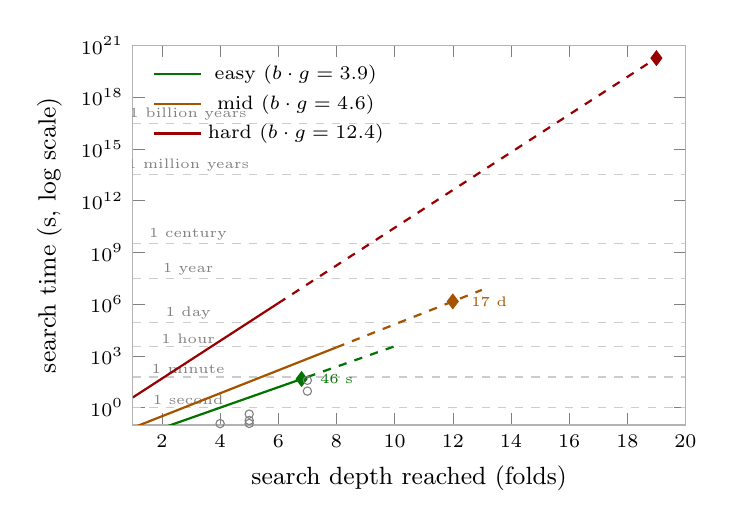
\begin{tikzpicture}
\begin{axis}[
  width=8.6cm, height=6.4cm,
  ymode=log,
  xlabel={search depth reached (folds)},
  ylabel={search time (s, log scale)},
  xmin=1, xmax=20, ymin=1e-1, ymax=1e21,
  xtick={2,4,6,8,10,12,14,16,18,20},
  ytick={1e0,1e3,1e6,1e9,1e12,1e15,1e18,1e21},
  tick label style={font=\scriptsize},
  label style={font=\small},
  legend style={font=\scriptsize, at={(0.02,0.98)}, anchor=north west, draw=none, fill=none},
  axis line style={gray!60},
]
\draw[gray!40, dashed, thin] (axis cs:1,1.0000e+0) -- (axis cs:20,1.0000e+0)
  node[pos=0.10, above, font=\tiny, gray, inner sep=1pt] {1 second};
\draw[gray!40, dashed, thin] (axis cs:1,6.0000e+1) -- (axis cs:20,6.0000e+1)
  node[pos=0.10, above, font=\tiny, gray, inner sep=1pt] {1 minute};
\draw[gray!40, dashed, thin] (axis cs:1,3.6000e+3) -- (axis cs:20,3.6000e+3)
  node[pos=0.10, above, font=\tiny, gray, inner sep=1pt] {1 hour};
\draw[gray!40, dashed, thin] (axis cs:1,8.6400e+4) -- (axis cs:20,8.6400e+4)
  node[pos=0.10, above, font=\tiny, gray, inner sep=1pt] {1 day};
\draw[gray!40, dashed, thin] (axis cs:1,3.1558e+7) -- (axis cs:20,3.1558e+7)
  node[pos=0.10, above, font=\tiny, gray, inner sep=1pt] {1 year};
\draw[gray!40, dashed, thin] (axis cs:1,3.1558e+9) -- (axis cs:20,3.1558e+9)
  node[pos=0.10, above, font=\tiny, gray, inner sep=1pt] {1 century};
\draw[gray!40, dashed, thin] (axis cs:1,3.1558e+13) -- (axis cs:20,3.1558e+13)
  node[pos=0.10, above, font=\tiny, gray, inner sep=1pt] {1 million years};
\draw[gray!40, dashed, thin] (axis cs:1,3.1558e+16) -- (axis cs:20,3.1558e+16)
  node[pos=0.10, above, font=\tiny, gray, inner sep=1pt] {1 billion years};
\addplot[thick, color=green!45!black, mark=none] coordinates {
  (1,1.66830e-2)
  (2,6.54005e-2)
  (3,2.56383e-1)
  (4,1.00507e+0)
  (5,3.94007e+0)
  (6,1.54458e+1)
  (7,6.05506e+1)
};
\addlegendentry{easy ($b\cdot g=3.9$)}
\addplot[thick, dashed, color=green!45!black, mark=none, forget plot] coordinates {
  (7,6.05506e+1)
  (8,2.37370e+2)
  (9,9.30537e+2)
  (10,3.64789e+3)
};
\addplot[thick, color=orange!65!black, mark=none] coordinates {
  (1,6.89243e-2)
  (2,3.19313e-1)
  (3,1.47932e+0)
  (4,6.85338e+0)
  (5,3.17504e+1)
  (6,1.47093e+2)
  (7,6.81456e+2)
  (8,3.15705e+3)
};
\addlegendentry{mid ($b\cdot g=4.6$)}
\addplot[thick, dashed, color=orange!65!black, mark=none, forget plot] coordinates {
  (8,3.15705e+3)
  (9,1.46260e+4)
  (10,6.77595e+4)
  (11,3.13917e+5)
  (12,1.45432e+6)
  (13,6.73756e+6)
};
\addplot[thick, color=red!60!black, mark=none] coordinates {
  (1,3.94464e+0)
  (2,4.88768e+1)
  (3,6.05619e+2)
  (4,7.50405e+3)
  (5,9.29805e+4)
  (6,1.15209e+6)
};
\addlegendentry{hard ($b\cdot g=12.4$)}
\addplot[thick, dashed, color=red!60!black, mark=none, forget plot] coordinates {
  (6,1.15209e+6)
  (7,1.42753e+7)
  (8,1.76881e+8)
  (9,2.19168e+9)
  (10,2.71564e+10)
  (11,3.36487e+11)
  (12,4.16932e+12)
  (13,5.16608e+13)
  (14,6.40114e+14)
  (15,7.93146e+15)
  (16,9.82765e+16)
  (17,1.21772e+18)
  (18,1.50884e+19)
  (19,1.86955e+20)
};
\addplot[only marks, mark=diamond*, mark size=2.6pt, color=green!45!black, forget plot]
  coordinates {(6.80,4.60741e+1)};
\node[font=\tiny, color=green!45!black, anchor=west] at (axis cs:7.10,4.60741e+1) {46 s};
\addplot[only marks, mark=diamond*, mark size=2.6pt, color=orange!65!black, forget plot]
  coordinates {(12.00,1.45432e+6)};
\node[font=\tiny, color=orange!65!black, anchor=west] at (axis cs:12.30,1.45432e+6) {17 d};
\addplot[only marks, mark=diamond*, mark size=2.6pt, color=red!60!black, forget plot]
  coordinates {(19.00,1.86955e+20)};

\addplot[only marks, mark=o, mark size=1.5pt, color=gray, forget plot] coordinates {
  (4,1.20000e-1)
  (5,4.25000e-1)
  (5,1.82000e-1)
  (5,1.23000e-1)
  (7,9.14900e+0)
  (7,3.87370e+1)
};
\end{axis}
\end{tikzpicture}
\caption{\textbf{Breadth-first search time against search depth, by difficulty group.}
The vertical axis is logarithmic, so a straight line is exponential growth and its slope is
$\log(b\cdot g)$. Curves are $t(d)=c_0(b\cdot g)^d$, the product of two exponentials: the
frontier grows as $b^d$ for a deduplicated branching factor $b$, measured as generated over
expanded during search, while the cost of expanding one node grows as $g^d$, because one
enumeration evaluates $4\times(\text{distinct crease lines})\times(\text{facets})$ candidates
and a fold of all layers at most doubles the facets. $g$ and $c_0$ are fitted by least squares
on per-depth enumeration timings. Each curve is solid only where that group was observed and
dashed beyond, and spans only the depths its own corpus reaches. Diamonds are each group's
mean reference depth; the hard group's sits at $10^{20}$ seconds, which is why the axis runs
that far. Circles are observed solves. $b$ is fitted from budget-exhausted runs: 7 over 3
samples for easy, 12 over 3 for medium, and 8 over 2 for hard, across 5 time budgets. The
hard extrapolation rests on two samples and is shown for its slope rather than for any value
it reaches.}
\label{fig:depth-wall}
\end{figure}


The supplementary cost model approximates search time as the product of two exponential factors:
the frontier grows with the branching factor, and the cost of expanding one node grows with depth
as well, because one enumeration evaluates four candidates per crease line per facet and a fold of
all layers at most doubles the facets. Fitting both from the saved searches gives a per-fold
multiplier of 3.9 on the easy group, 4.6 on medium and 12.4 on hard
(Figure~\ref{fig:depth-wall}). These fitted curves extrapolate beyond the observed depths; they are not measured
solution times or lower bounds. The hard-group fit uses only two samples, so its factor is
illustrative only; because depth is confounded with layer and crease count across groups, none of
the fitted factors should be read as the intrinsic complexity of the task. No matched, fixed-budget comparison of
search and models on the same instances has been run.
% EDITING NOTE: Validate the cost model and extrapolations before submission.


% Source: workspace/RESULTS/results.md, Deterministic search baseline.
% Static TeX bars; no additional plotting package or runtime required.
\begin{figure}[t]
\centering
\small
\begin{tabular}{llr}
Group (reference folds) & Median states expanded & Solved / attempts \\
\hline
Easy (4--10) & \rule{0.247cm}{8pt}\quad 65 & 366/669 \\
Medium (11--13) & \rule{4cm}{8pt}\quad 1,051.5 & 1/40 \\
Hard (14--19) & \rule{2.024cm}{8pt}\quad 532 & 0/16 \\
\end{tabular}
\caption{Observed BFS search effort in the saved aggregate. Bar lengths use a linear scale and
show median states expanded across attempts, including unsuccessful attempts. Budgets and repeated
samples are not standardized by this aggregate; 358 of 725 attempts terminated in timeout.
}
\label{fig:bfs-effort}
\end{figure}



\subsection{Dataset generation}
\label{app:generation-procedure}

{\small\begin{verbatim}
GENERATE(reference_depth, action_model):
    state <- unfolded square
    actions, frames <- [], []
    for step in 1..reference_depth:
        candidates <- LEGAL_FOLDS(state, action_model)
        if candidates is empty: return FAILED
        action <- SAMPLE(candidates)
        state <- APPLY(state, action)
        actions.append(action)
        frames.append(state)
    cp <- CREASE_PATTERN_IN_ORIGINAL_SHEET(state)
    cp <- SPLIT_EDGES_AT_INTERSECTIONS(cp)
    if not REPLAY_CHECK(cp, actions, state): return FAILED
    return (cp, state, actions, frames, METADATA(actions))
\end{verbatim}
}

\subsection{Evaluation pipeline}
\label{app:evaluation-pipeline}

{\small\begin{verbatim}
EPISODE(sample, model, condition, query_budget):
    cp, target <- LOAD_INPUTS(sample)
    session <- INITIALIZE(cp, target, unfolded_square)
    history <- []
    for query in 1..query_budget:
        obs <- OBSERVE(session, condition)
        call <- model(cp, target, obs, history, condition)
        if call is finish: break
        # Edits: add/remove fold, go to step, restore revision.
        # Reads: state, images, candidates, target feedback.
        result <- DISPATCH_TRANSACTIONALLY(session, call)
        # Rejected edits leave session unchanged but consume a query.
        # Read calls consume a query without changing the sequence.
        history.append(call, result)
        if STOPPING_RULE(session, history): break
    return SCORE(REPLAY(session.actions), REFERENCE_AT_SCORING(sample))
\end{verbatim}
}

\begin{figure}[t]
\centering
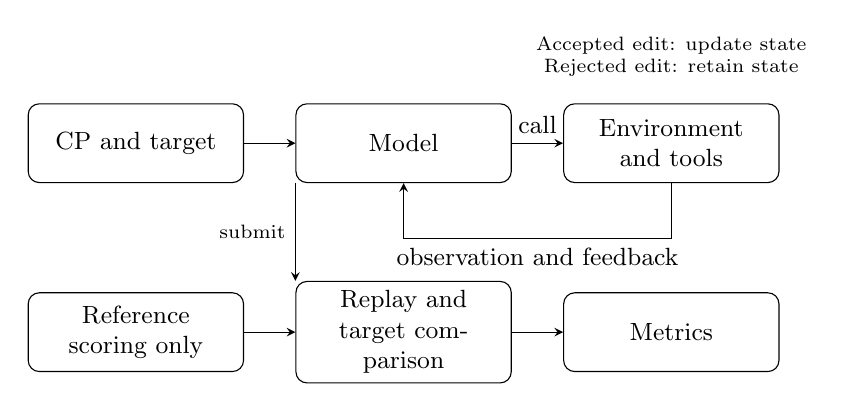
\begin{tikzpicture}[font=\small,box/.style={draw,rounded corners,align=center,text width=2.5cm,minimum height=1cm},>=stealth]
\node[box] (input) at (0,0) {CP and target};
\node[box] (model) at (3.4,0) {Model};
\node[box] (env) at (6.8,0) {Environment\\and tools};
\draw[->] (input)--(model);
\draw[->] (model)--node[above]{call}(env);
\draw[->] (env.south) -- ++(0,-.7) -| node[pos=.25,below]{observation and feedback}(model.south);
\node[align=center,font=\scriptsize] at (6.8,1.1) {Accepted edit: update state\\Rejected edit: retain state};
\node[box] (score) at (3.4,-2.4) {Replay and\\target comparison};
\node[box] (ref) at (0,-2.4) {Reference\\scoring only};
\node[box] (metrics) at (6.8,-2.4) {Metrics};
\draw[->] (model.south west)--node[left,font=\scriptsize]{submit}(score.north west);
\draw[->] (ref)--(score);
\draw[->] (score)--(metrics);
\end{tikzpicture}
\caption{Evaluation pipeline. The model edits and inspects its current construction. The reference
sequence is withheld from the model and used only for scoring.}
\label{fig:pipeline}
\end{figure}


\subsection{Tool interface and feedback}
\label{app:tool-interface}
Basic tools comprise all entries in Table~\ref{tab:tools} except the optional
\texttt{list\_legal\_folds} and \texttt{compare\_to\_target} tools.
Loading and configuration are described in Appendix~\ref{app:tool-loading}.

\begin{table}[h]
\centering
\caption{Tools available to the evaluation harness; exposure depends on run configuration.}
\label{tab:tools}
\begin{tabular}{lp{0.65\textwidth}}
\hline
Tool & Operation \\
\hline
\texttt{add\_fold} & Append a checked fold; reject invalid actions without changing state. \\
\texttt{remove\_fold} & Remove a specified fold and replay the remainder transactionally. \\
\texttt{go\_to\_step} & Retain the first specified number of folds. \\
\texttt{restore\_revision} & Restore a previously recorded branch state. \\
\texttt{get\_state} & Return the current sequence and layer geometry. \\
\texttt{get\_images} & Render top, oblique, reverse, X-ray, and exploded views of a completed step; exposed views depend on run configuration. \\
\texttt{list\_legal\_folds} & Optionally enumerate legal candidates compatible with the target CP. \\
\texttt{compare\_to\_target} & Optionally return feedback at the configured level (Section~\ref{sec:target-feedback}). \\
\texttt{finish} & End the episode and evaluate the current sequence. \\
\hline
\end{tabular}
\end{table}

\subsubsection{Target-feedback levels}
\label{app:feedback-levels}
The run configuration selects one of three feedback levels for
\texttt{compare\_to\_target}. The tool compares the current and target stacks.

\begin{table}[h]
\centering
\caption{Information returned at each target-feedback level.}
\begin{tabular}{lp{0.72\textwidth}}
\hline
Level & Information returned \\
\hline
1: Counts & Current and target layer counts, their difference, and a count-based summary. \\
2: Diagnosis & Level 1 plus aligned layer matches, mismatched ranks, and a diagnosis of count,
shape, orientation, or ordering disagreement. \\
3: Corrections & Level 2 plus suggested corrections for up to twelve mismatched ranks, such as
orientation changes or a different target rank for a layer shape. \\
\hline
\end{tabular}
\end{table}

\subsection{Tool schemas and prompt}
The following listings document the tool schemas and folding prompt; tool exposure is configured per run.
\lstinputlisting{listings/tool_schemas.py}
\lstinputlisting{listings/fold_prompt.md}

\subsection{Sample contents}
\label{app:sample-contents}
Each sample contains the input crease pattern, a reference state sequence, reference
fold actions, and metadata (Table~\ref{tab:sample-files}).

\begin{table}[h]
\centering
\caption{Contents of a CP2Seq sample.}
\label{tab:sample-files}
\label{sec:cp2seq-sample}
\begin{tabular}{lp{0.68\textwidth}}
\hline
Artifact & Contents \\
\hline
Crease pattern & Input crease geometry. \\
State sequence & Folded states after each reference action; only the final state is supplied
as the target. \\
Reference actions & Withheld fold lines, directions, layer selections, and
creases created. \\
Metadata & Sample descriptors and generator version. \\
\hline
\end{tabular}
\end{table}

\subsection{Dataset gallery and reference sequences}
Each rendered panel contains the crease pattern, top view, and an oblique view with illustrative
layer separation.
\IfFileExists{figures/dataset/gallery.tex}{\noindent all-layers/easy-0001 (all-layers, 4 reference folds)\par
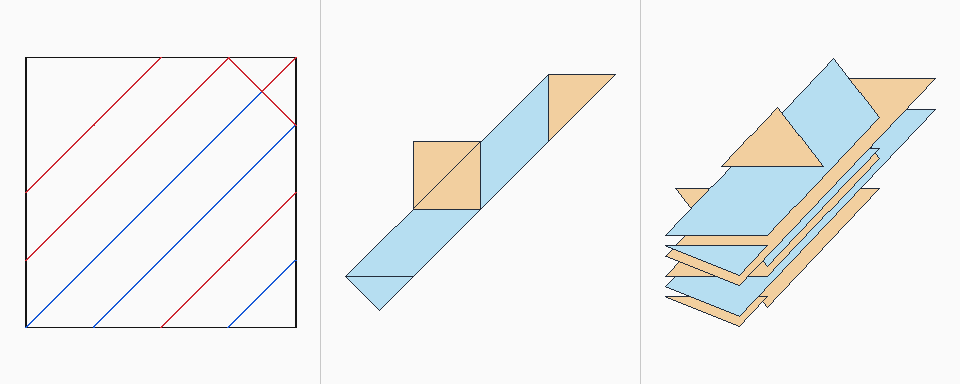
\includegraphics[width=\linewidth]{figures/dataset/sample-1.png}\par\medskip
\noindent all-layers/mid-0004 (all-layers, 11 reference folds)\par
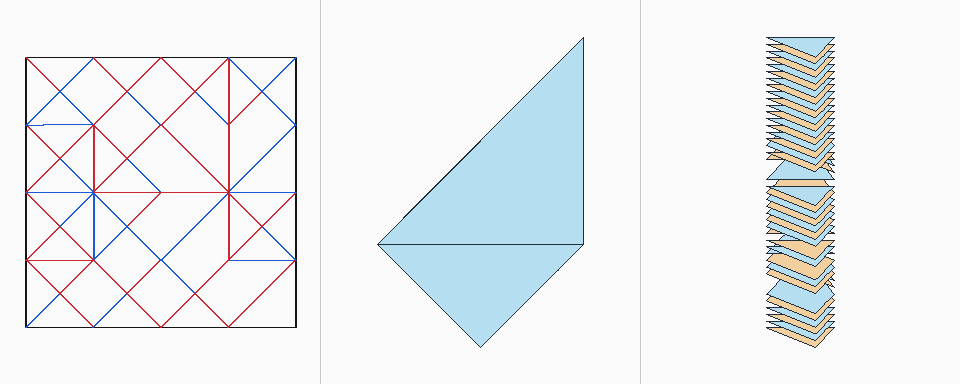
\includegraphics[width=\linewidth]{figures/dataset/sample-2.png}\par\medskip
\noindent some-generated-d5/layers-0001 (some-layers, 5 reference folds)\par
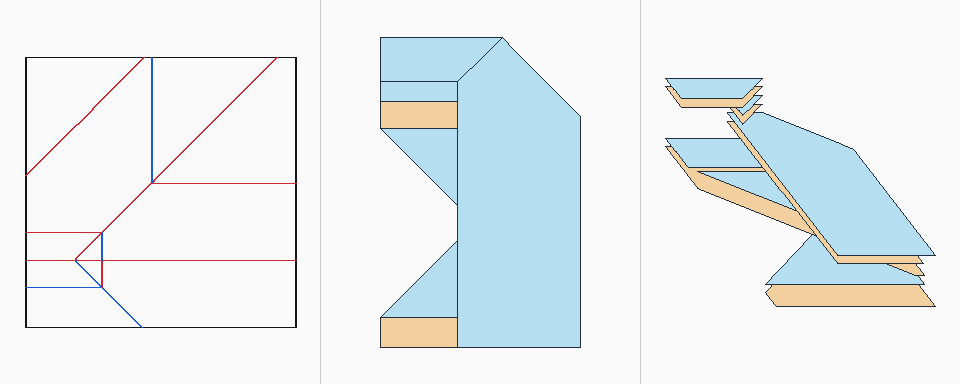
\includegraphics[width=\linewidth]{figures/dataset/sample-3.png}\par\medskip
\noindent all-layers/hard-0004 (all-layers, 15 reference folds)\par
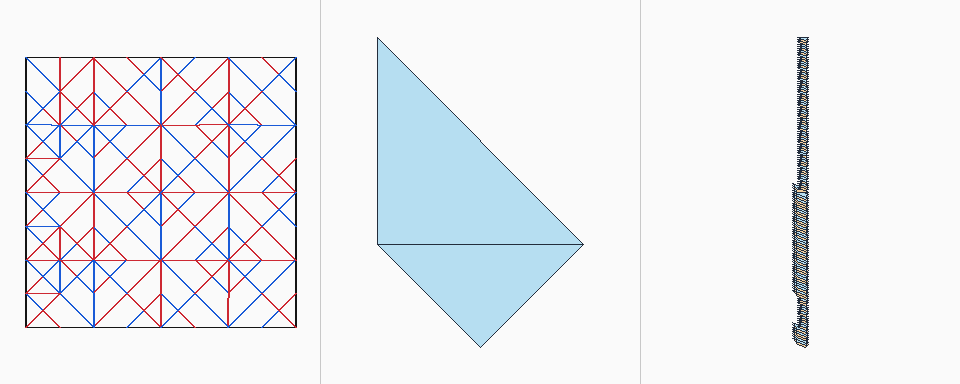
\includegraphics[width=\linewidth]{figures/dataset/sample-4.png}\par\medskip
\noindent all-layers/hard-0005 (all-layers, 15 reference folds)\par
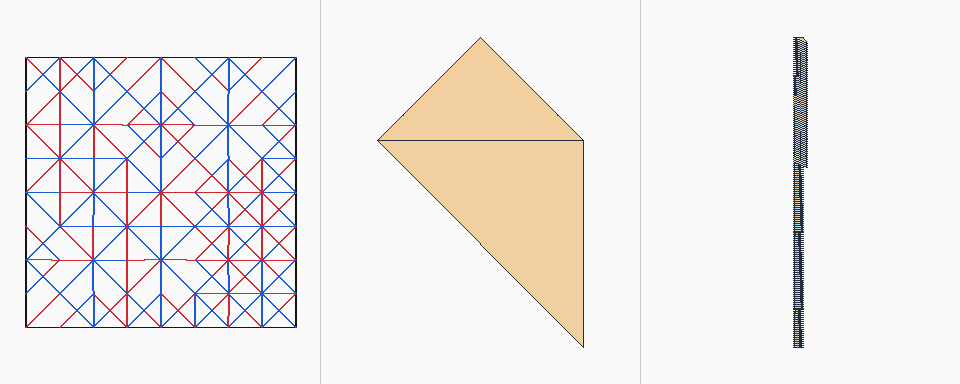
\includegraphics[width=\linewidth]{figures/dataset/sample-5.png}\par\medskip
\noindent all-layers/hard-0006 (all-layers, 15 reference folds)\par
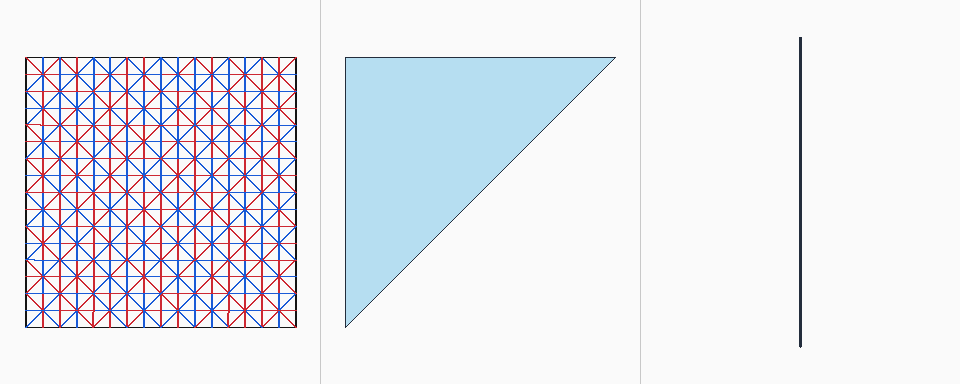
\includegraphics[width=\linewidth]{figures/dataset/sample-6.png}\par\medskip
}{
\noindent\fbox{\parbox{.9\linewidth}{Dataset gallery pending export: short all-layers,
longer all-layers, and some-layers examples.}}}
\IfFileExists{figures/dataset/sequences.tex}{\paragraph{all-layers/easy-0001 (all-layers, 4 reference folds)}
\noindent Stored state 0\par
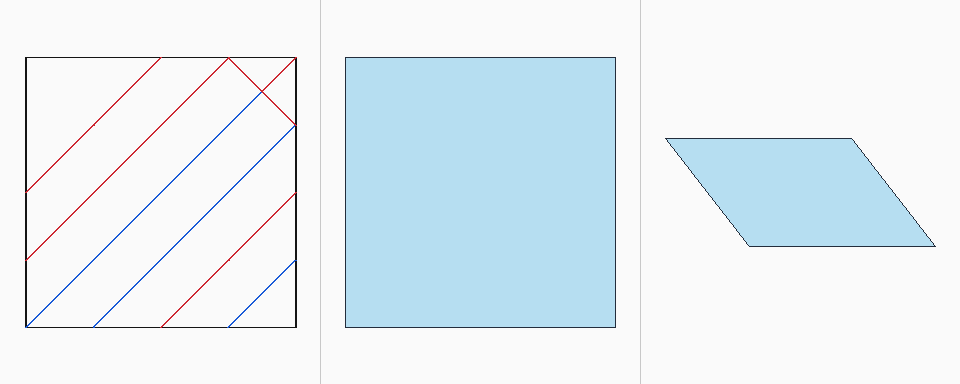
\includegraphics[width=.72\linewidth]{figures/dataset/sample-1-state-0.png}\par
\noindent Stored state 1\par
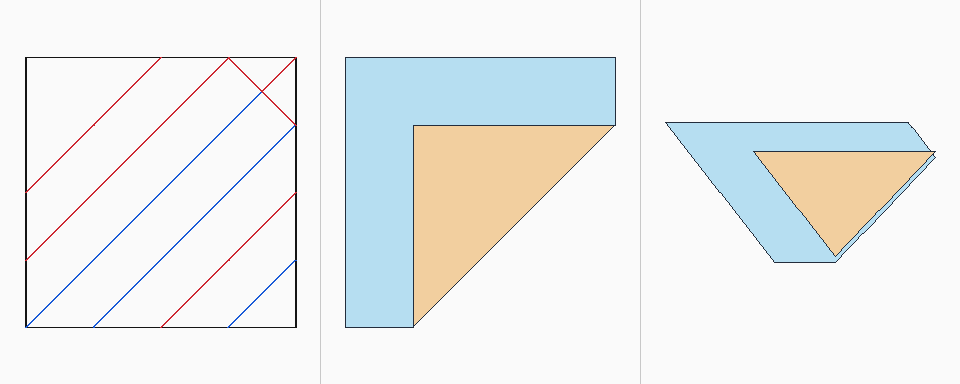
\includegraphics[width=.72\linewidth]{figures/dataset/sample-1-state-1.png}\par
\noindent Stored state 2\par
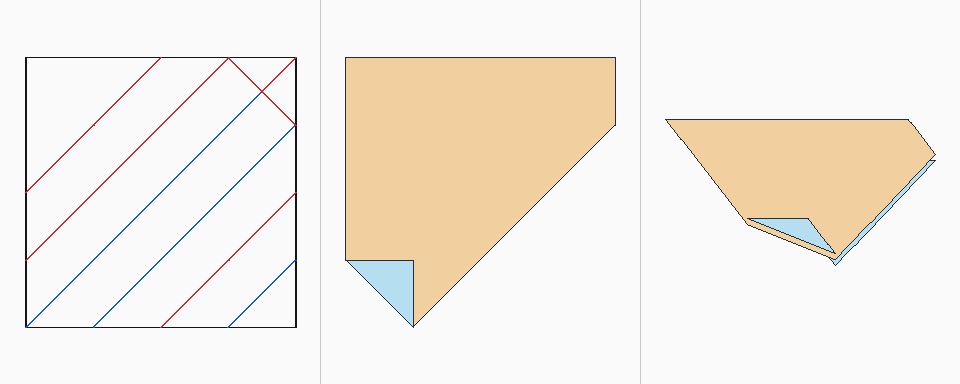
\includegraphics[width=.72\linewidth]{figures/dataset/sample-1-state-2.png}\par
\noindent Stored state 3\par
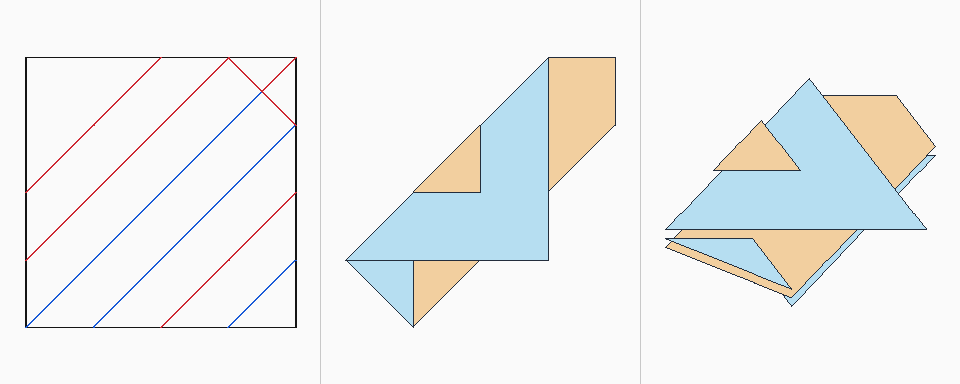
\includegraphics[width=.72\linewidth]{figures/dataset/sample-1-state-3.png}\par
\noindent Stored state 4\par
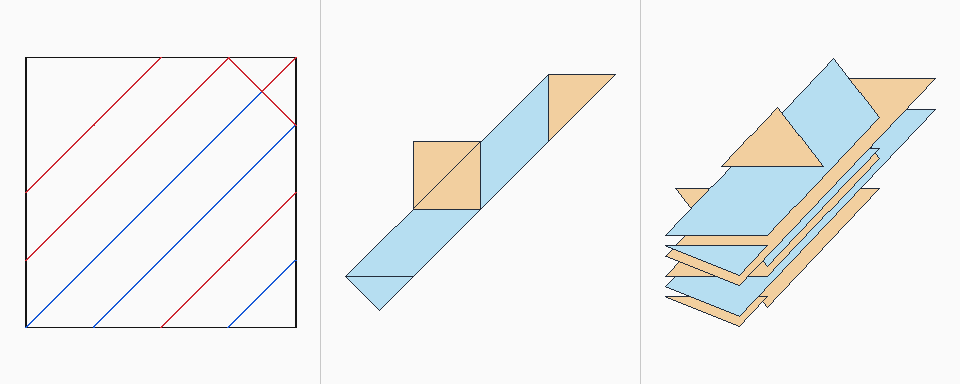
\includegraphics[width=.72\linewidth]{figures/dataset/sample-1-state-4.png}\par
\paragraph{all-layers/mid-0004 (all-layers, 11 reference folds)}
\noindent Stored state 0\par
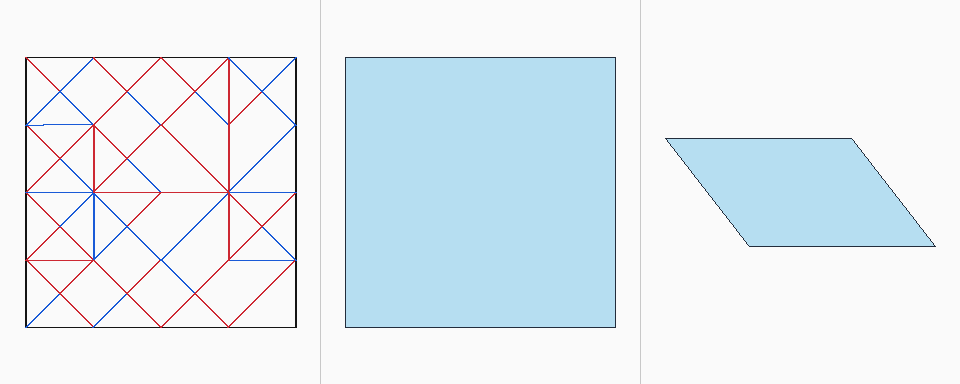
\includegraphics[width=.72\linewidth]{figures/dataset/sample-2-state-0.png}\par
\noindent Stored state 1\par
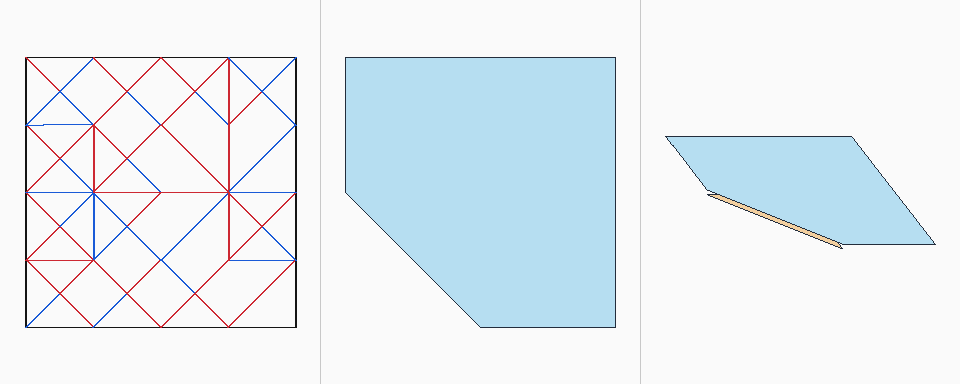
\includegraphics[width=.72\linewidth]{figures/dataset/sample-2-state-1.png}\par
\noindent Stored state 2\par
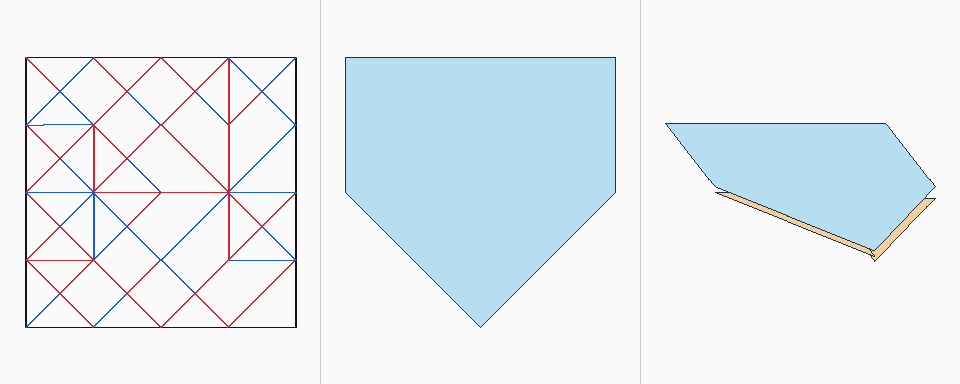
\includegraphics[width=.72\linewidth]{figures/dataset/sample-2-state-2.png}\par
\noindent Stored state 3\par
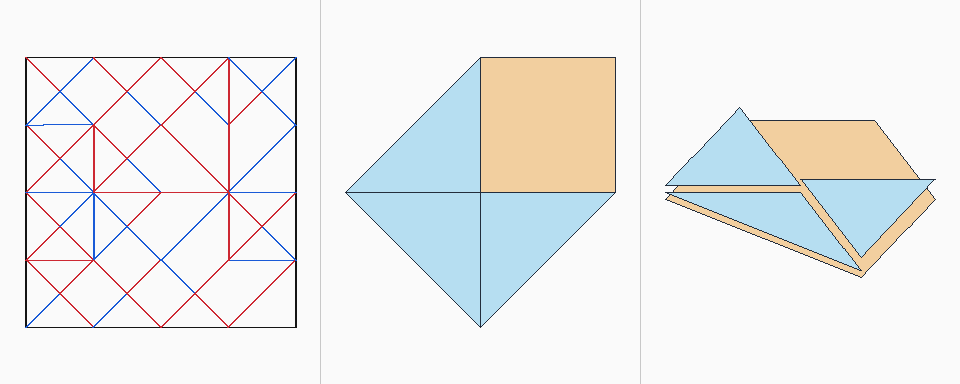
\includegraphics[width=.72\linewidth]{figures/dataset/sample-2-state-3.png}\par
\noindent Stored state 4\par
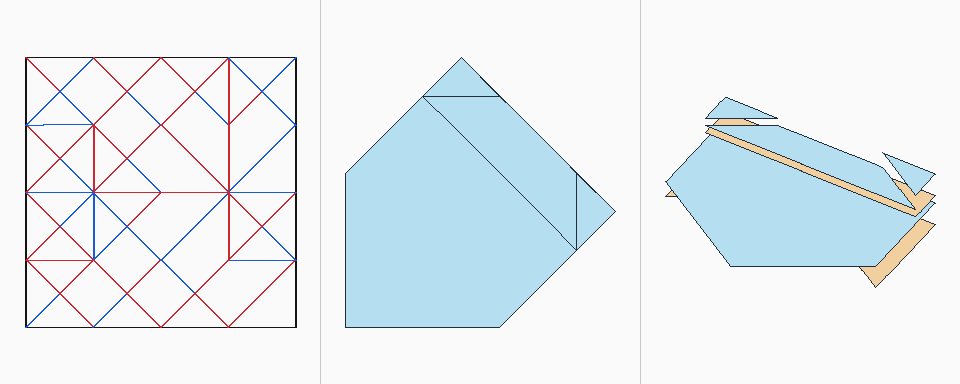
\includegraphics[width=.72\linewidth]{figures/dataset/sample-2-state-4.png}\par
\noindent Stored state 5\par
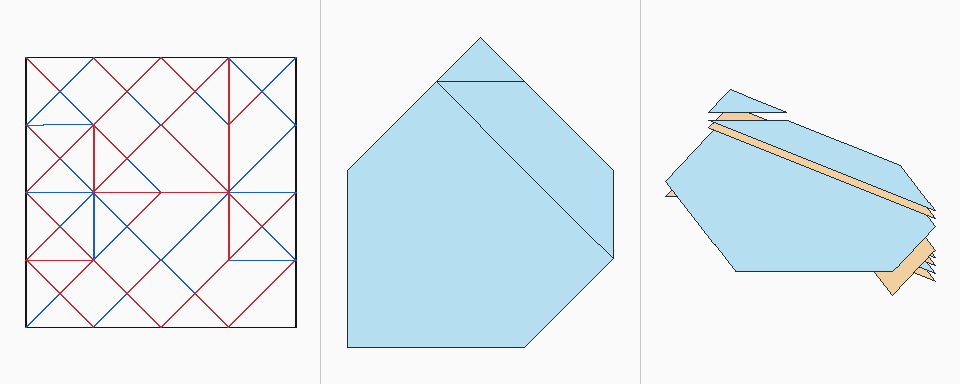
\includegraphics[width=.72\linewidth]{figures/dataset/sample-2-state-5.png}\par
\noindent Stored state 6\par
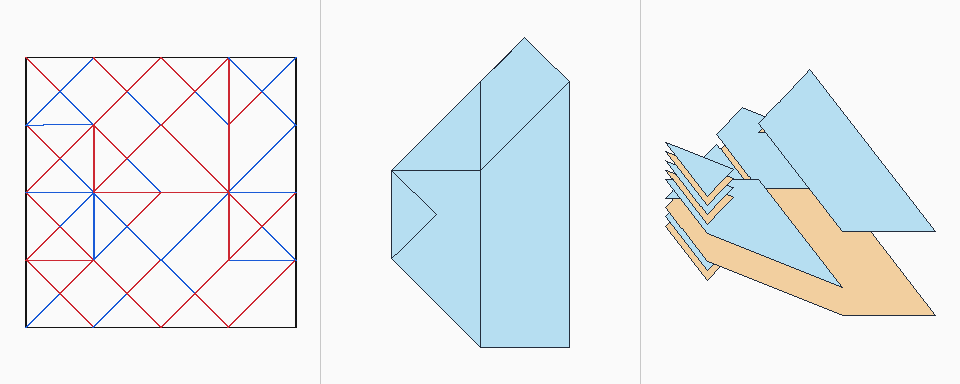
\includegraphics[width=.72\linewidth]{figures/dataset/sample-2-state-6.png}\par
\noindent Stored state 7\par
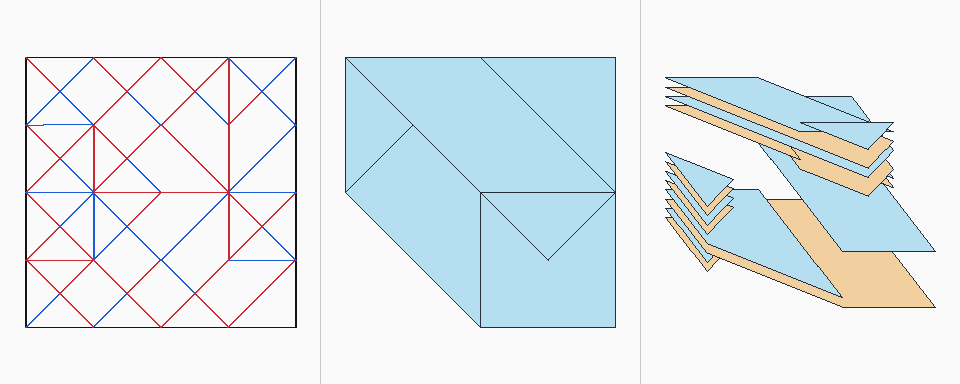
\includegraphics[width=.72\linewidth]{figures/dataset/sample-2-state-7.png}\par
\noindent Stored state 8\par
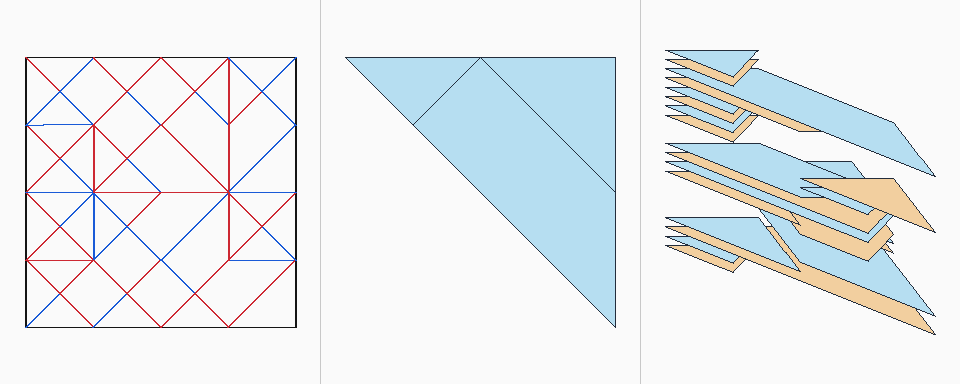
\includegraphics[width=.72\linewidth]{figures/dataset/sample-2-state-8.png}\par
\noindent Stored state 9\par
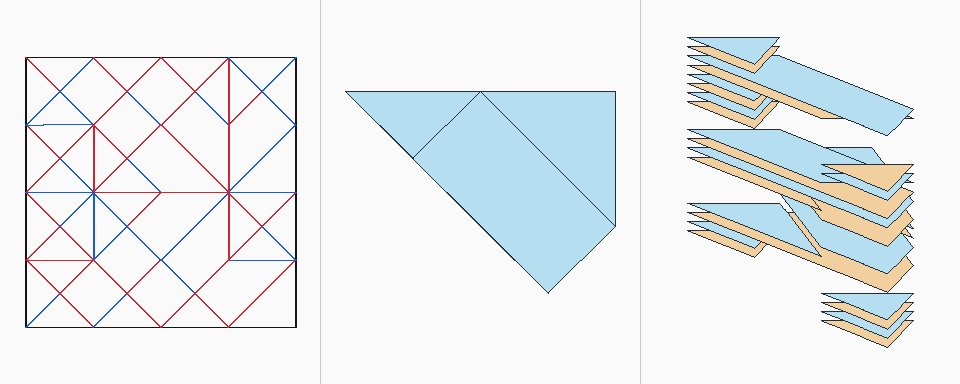
\includegraphics[width=.72\linewidth]{figures/dataset/sample-2-state-9.png}\par
\noindent Stored state 10\par
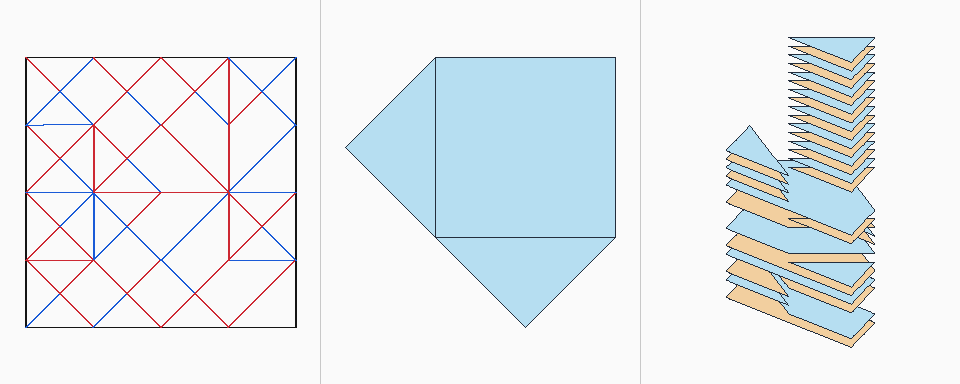
\includegraphics[width=.72\linewidth]{figures/dataset/sample-2-state-10.png}\par
\noindent Stored state 11\par
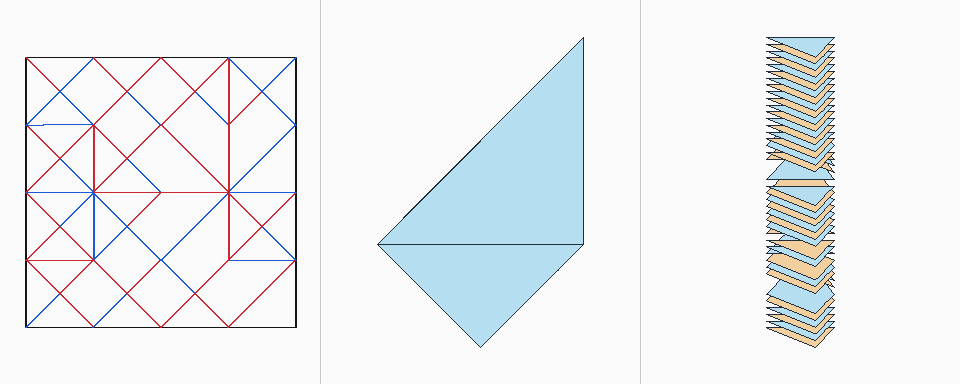
\includegraphics[width=.72\linewidth]{figures/dataset/sample-2-state-11.png}\par
\paragraph{some-generated-d5/layers-0001 (some-layers, 5 reference folds)}
\noindent Stored state 0\par
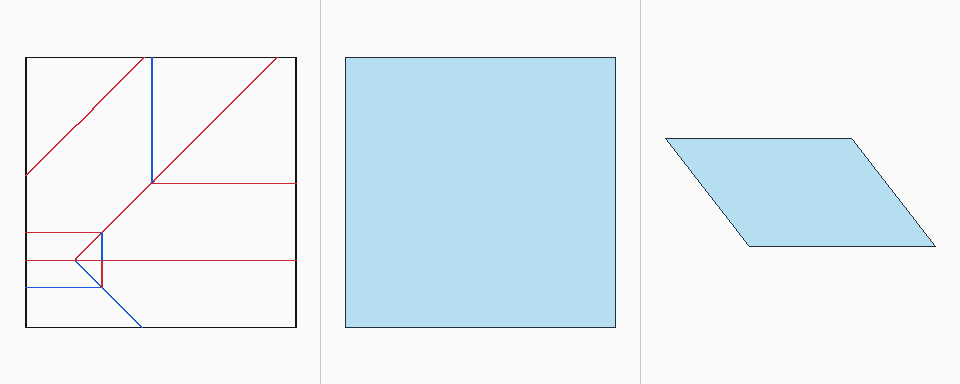
\includegraphics[width=.72\linewidth]{figures/dataset/sample-3-state-0.png}\par
\noindent Stored state 1\par
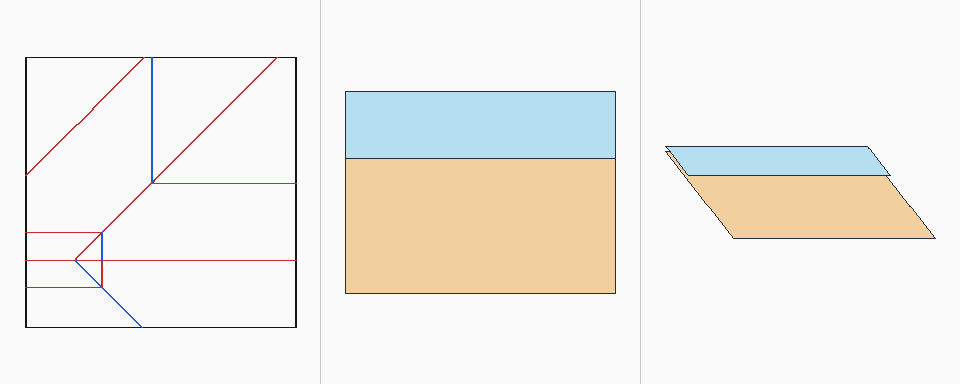
\includegraphics[width=.72\linewidth]{figures/dataset/sample-3-state-1.png}\par
\noindent Stored state 2\par
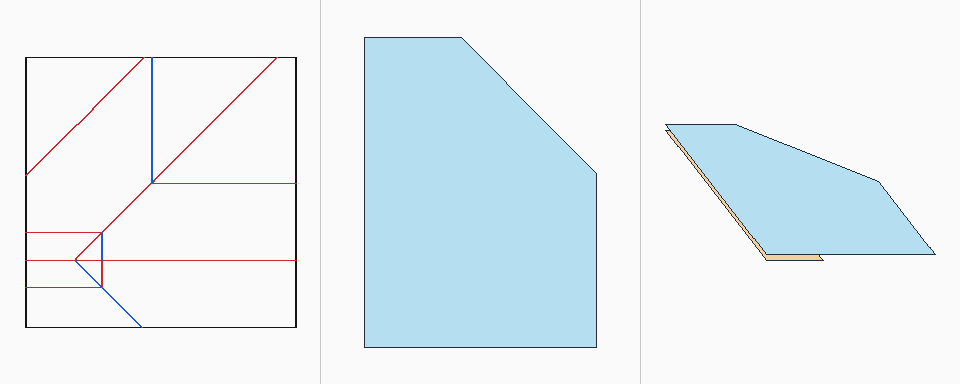
\includegraphics[width=.72\linewidth]{figures/dataset/sample-3-state-2.png}\par
\noindent Stored state 3\par
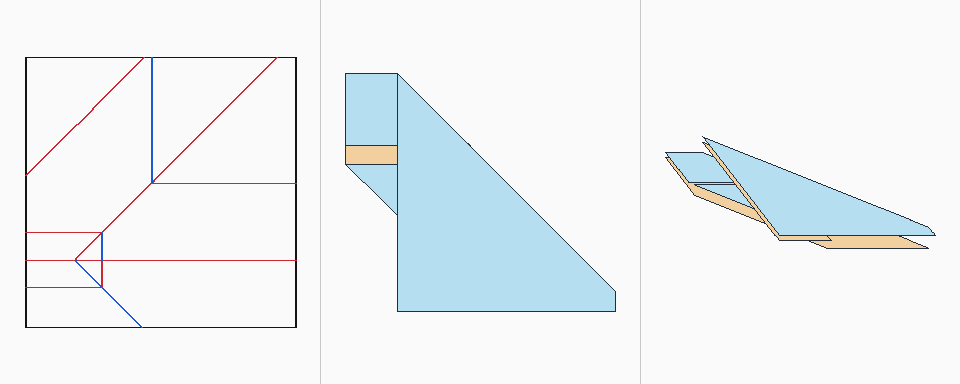
\includegraphics[width=.72\linewidth]{figures/dataset/sample-3-state-3.png}\par
\noindent Stored state 4\par
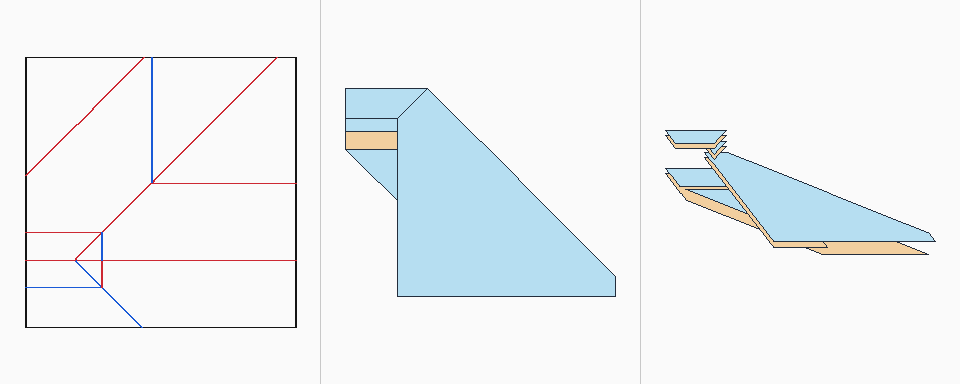
\includegraphics[width=.72\linewidth]{figures/dataset/sample-3-state-4.png}\par
\noindent Stored state 5\par
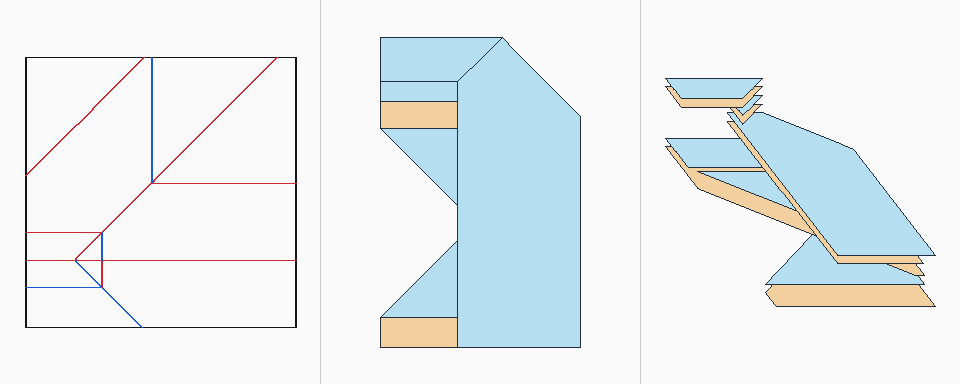
\includegraphics[width=.72\linewidth]{figures/dataset/sample-3-state-5.png}\par
}{}

\subsection{Trace-analysis interface}
We provide a trace-inspection interface for browsing saved runs, replaying recorded folding
trajectories, and examining model actions alongside tool feedback and rendered states. This
supports qualitative analysis of successful construction, repeated exploration, and unsuccessful
termination. A command-line trace viewer additionally supports filtering by task, trial,
session, role, and event type.

Figures~\ref{fig:dataset-browser-ui} and~\ref{fig:trace-viewer-ui} show the dataset
browser and trace viewer, respectively. These interfaces support inspection of
reference sequences and recorded model episodes.

\begin{figure}[tbp]
\centering
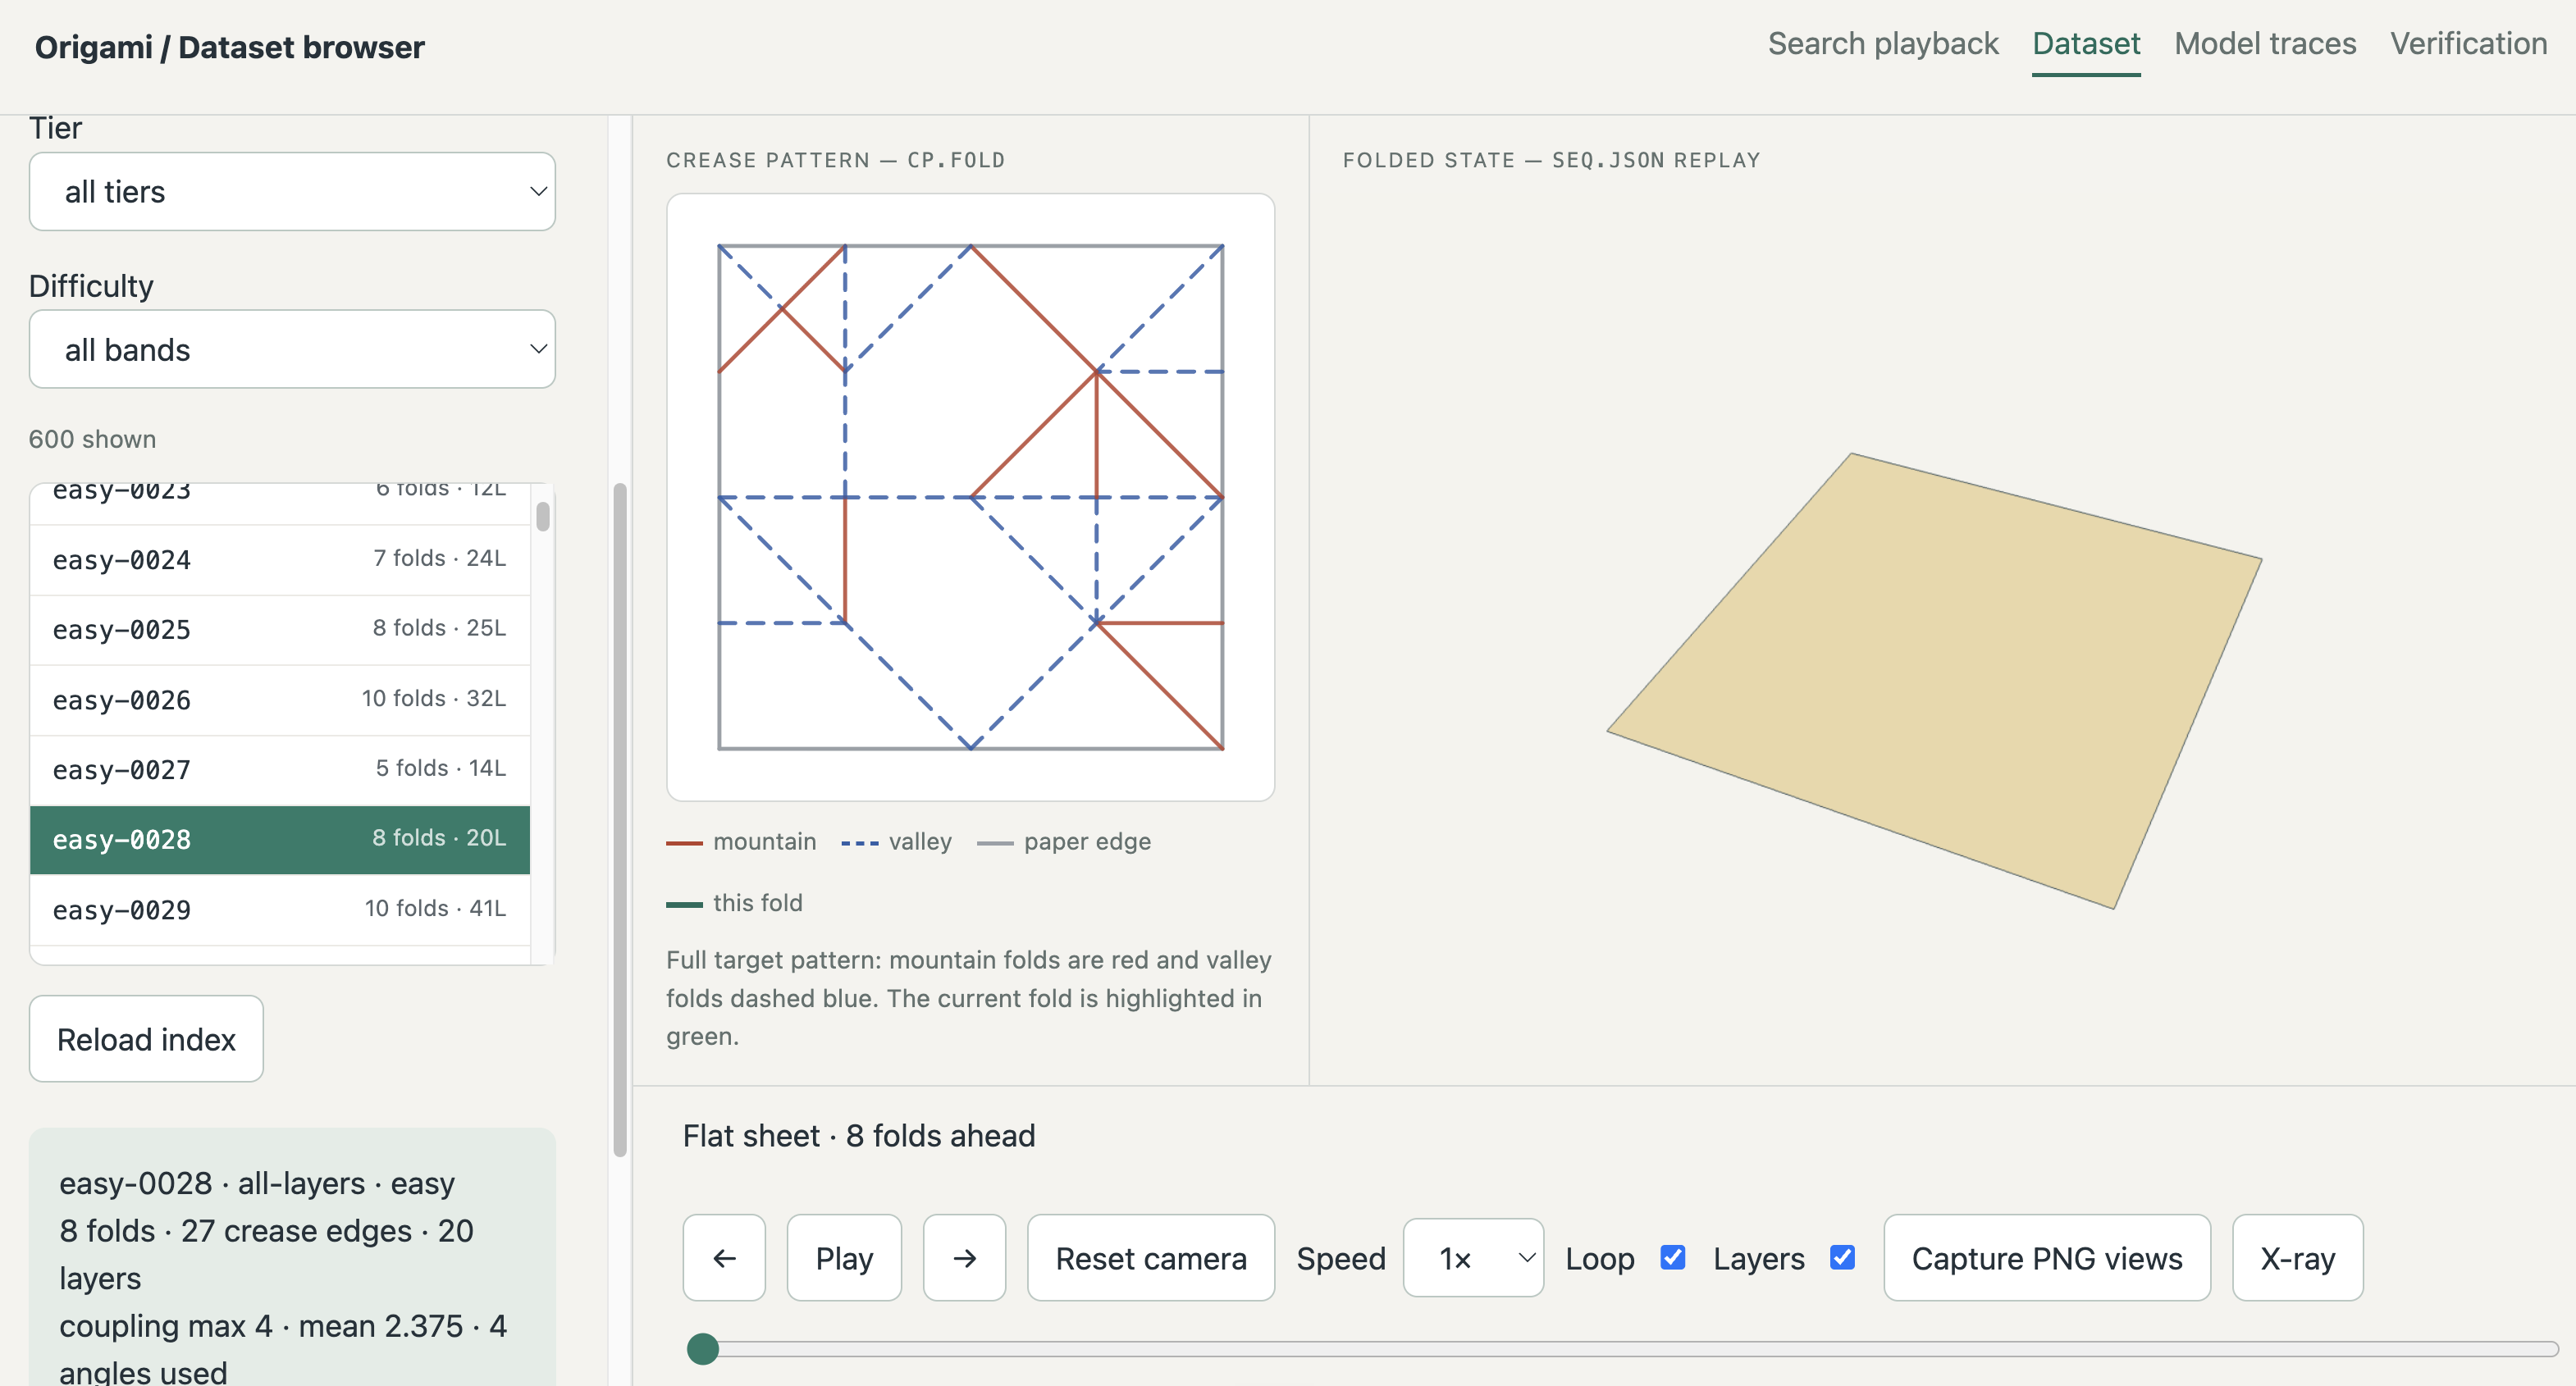
\includegraphics[width=\linewidth,height=.34\textheight,keepaspectratio]{figures/screenshots/dataset-browser.png}
\caption{Dataset browser with \texttt{easy-0028} selected. The interface displays
sample metadata, the target crease pattern, and reference-sequence playback controls.
The right panel shows the unfolded sheet at step zero.}
\label{fig:dataset-browser-ui}
\end{figure}

\begin{figure}[tbp]
\centering
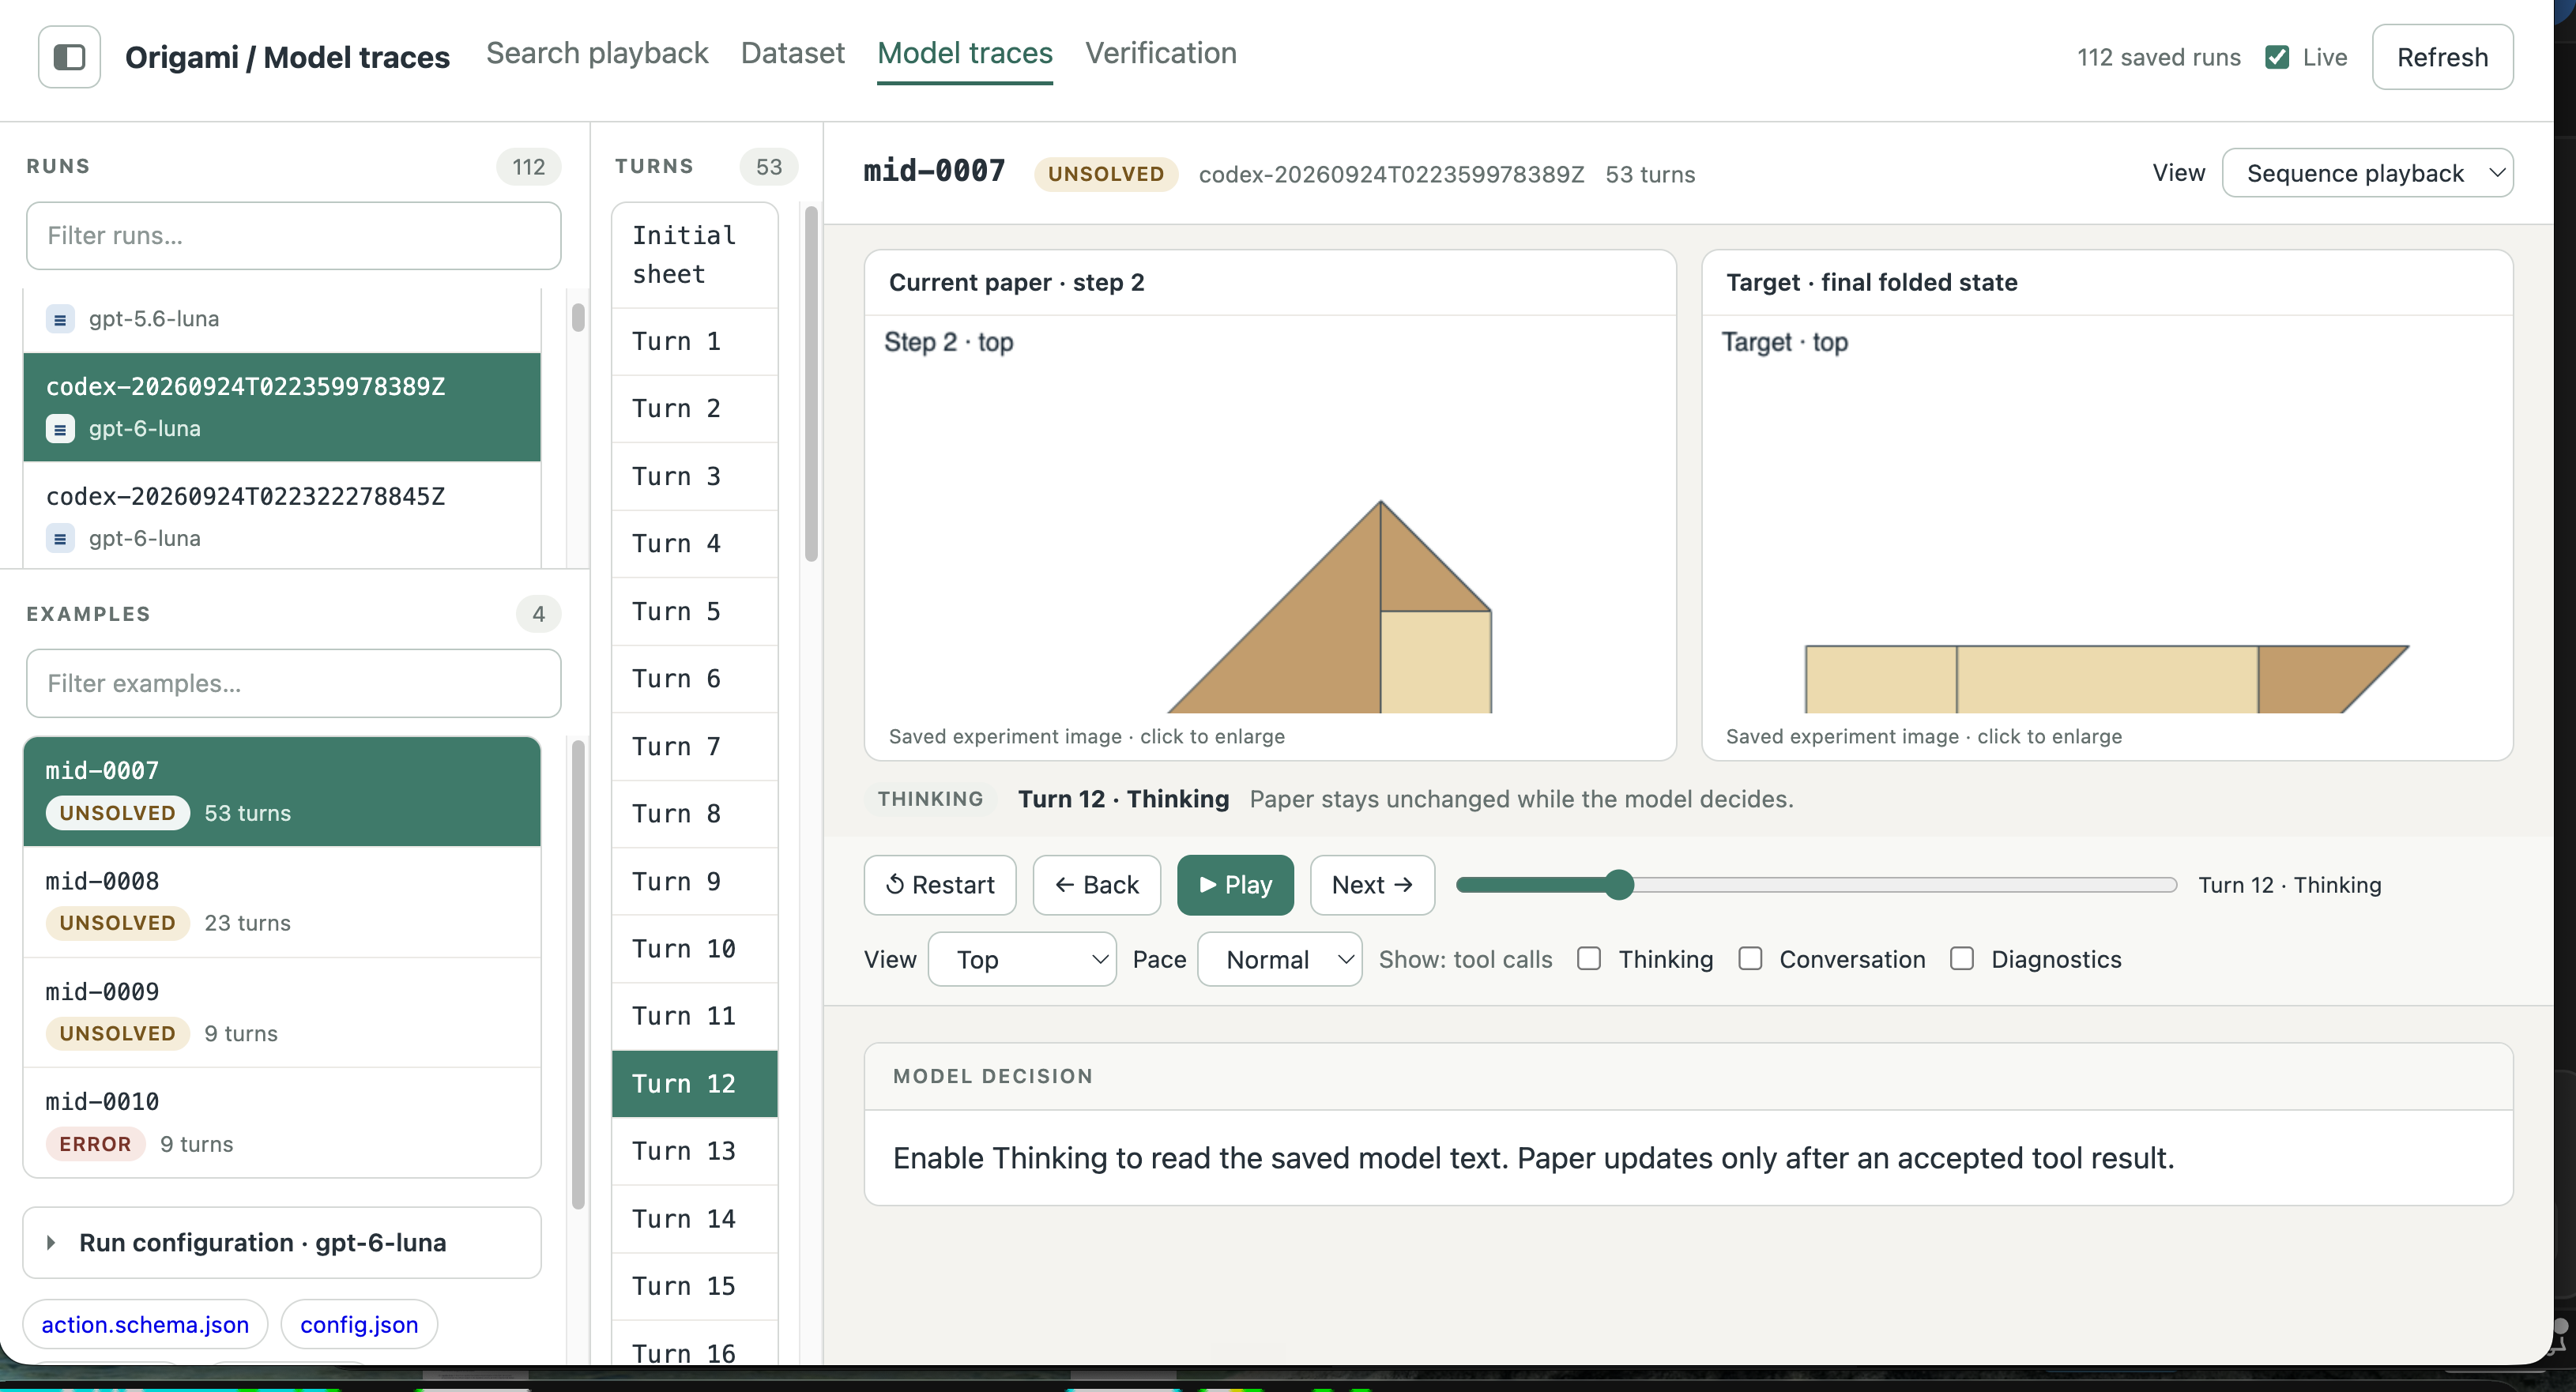
\includegraphics[width=\linewidth,height=.34\textheight,keepaspectratio]{figures/screenshots/trace-viewer.png}
\caption{Trace viewer for a saved GPT-6 Luna attempt on \texttt{mid-0007}.
Run and turn navigation appear beside the current and target states. The selected
episode is marked unsolved; the displayed frame is at turn 12. Playback controls allow inspection of saved actions
and feedback.}
\label{fig:trace-viewer-ui}
\end{figure}

% EDITING NOTE: 07.44.33 is a second dataset-browser capture, not a verification
% capture; retained in assets/screenshots but omitted as redundant. Add an actual
% Verification-tab capture when available. Screenshots above are user-provided.

% EDITING NOTE: Select actual saved episodes after inspecting their terminal verdicts.
% Include one solved, one cycling, and one unsuccessful non-cycling attempt. For each,
% give run/sample IDs, configuration, terminal reason, and selected actions/tool responses.
% Include screenshots from traces.html: target/current state plus action and feedback panes.
% Include actual request/response excerpts; do not invent representative tool responses.
% Attach per-run budgets, effort, tool schemas, comparison tier, and supplementary results.

\subsection{Tool loading and configuration}
\label{app:tool-loading}
The schema builder selects the tools exposed in each run. Basic mode excludes candidate
enumeration; filtered mode includes it. Target comparison is added only when a comparison level
is configured. For an all-layers action model, partial-layer selection arguments are removed
from the exposed action schemas. The run configuration therefore records tool mode, comparison
level, and action model separately.

% REFUSAL FIGURE PLAN: Use a saved some-layers would-tear response with geometric diagnostics.
\subsection{Rejection feedback}
Figure~\ref{fig:rejection-feedback} illustrates the geometric evidence associated with
a \texttt{would-tear} response using the shared verification fixtures. The comparison
holds the initial state and hinge fixed and changes the selected layers. The export
script records both engine responses and checks that rejection preserves the state.
\begin{figure}[tbp]
\centering
\IfFileExists{figures/rejection-feedback-panels.tex}{
  \begin{minipage}[t]{.47\linewidth}
\centering
\textbf{(a) Rejected proposal}\par\smallskip
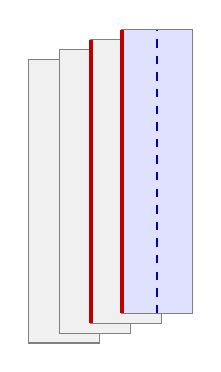
\begin{tikzpicture}[x=3.6cm,y=3.6cm,font=\scriptsize]
\draw[fill=gray!12,draw=gray] (0.000000,0.000000) -- (0.250000,0.000000) -- (0.250000,1.000000) -- (0.000000,1.000000) -- cycle;
\draw[fill=gray!12,draw=gray] (0.360000,0.035000) -- (0.110000,0.035000) -- (0.110000,1.035000) -- (0.360000,1.035000) -- cycle;
\draw[fill=gray!12,draw=gray] (0.220000,0.070000) -- (0.345000,0.070000) -- (0.470000,0.070000) -- (0.470000,1.070000) -- (0.345000,1.070000) -- (0.220000,1.070000) -- cycle;
\draw[fill=blue!12,draw=gray] (0.580000,0.105000) -- (0.455000,0.105000) -- (0.330000,0.105000) -- (0.330000,1.105000) -- (0.455000,1.105000) -- (0.580000,1.105000) -- cycle;
\draw[blue!75!black,dashed,thick] (0.455000,0.105000) -- (0.455000,1.105000);
\draw[red!75!black,line width=1.5pt] (0.330000,0.105000) -- (0.330000,1.105000);
\draw[red!75!black,line width=1.5pt] (0.220000,0.070000) -- (0.220000,1.070000);
\end{tikzpicture}\par
\texttt{would-tear}\par Top leaf selected; state unchanged.
\end{minipage}
\hfill
\begin{minipage}[t]{.47\linewidth}
\centering
\textbf{(b) Accepted proposal}\par\smallskip
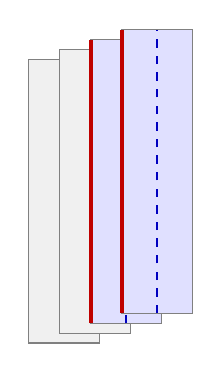
\begin{tikzpicture}[x=3.6cm,y=3.6cm,font=\scriptsize]
\draw[fill=gray!12,draw=gray] (0.000000,0.000000) -- (0.250000,0.000000) -- (0.250000,1.000000) -- (0.000000,1.000000) -- cycle;
\draw[fill=gray!12,draw=gray] (0.360000,0.035000) -- (0.110000,0.035000) -- (0.110000,1.035000) -- (0.360000,1.035000) -- cycle;
\draw[fill=blue!12,draw=gray] (0.220000,0.070000) -- (0.345000,0.070000) -- (0.470000,0.070000) -- (0.470000,1.070000) -- (0.345000,1.070000) -- (0.220000,1.070000) -- cycle;
\draw[blue!75!black,dashed,thick] (0.345000,0.070000) -- (0.345000,1.070000);
\draw[fill=blue!12,draw=gray] (0.580000,0.105000) -- (0.455000,0.105000) -- (0.330000,0.105000) -- (0.330000,1.105000) -- (0.455000,1.105000) -- (0.580000,1.105000) -- cycle;
\draw[blue!75!black,dashed,thick] (0.455000,0.105000) -- (0.455000,1.105000);
\draw[red!75!black,line width=1.5pt] (0.330000,0.105000) -- (0.330000,1.105000);
\draw[red!75!black,line width=1.5pt] (0.220000,0.070000) -- (0.220000,1.070000);
\end{tikzpicture}\par
\texttt{ok: true}\par Connected top pair selected.
\end{minipage}

}{
  \fbox{\parbox{.9\linewidth}{\small Rejection-feedback figure pending local export.
  Run \texttt{node workspace/export\_rejection\_figure.mjs} from the repository root.
  The exporter checks rejected and accepted proposals from the same four-layer state
  before writing the panels and response evidence.}}
}
\caption{Rejection feedback and a legal alternative from the same state. Dashed blue
lines mark the proposed hinge; red segments mark the shared material edge identified
by the tearing diagnostic. Blue shading identifies selected layers. Selecting only
the top leaf would separate it from its connected neighbour away from the hinge;
selecting the connected top pair permits the fold. Both panels show the pre-action
state, with illustrative layer separation. The example is rendered from verification fixtures.}
\label{fig:rejection-feedback}
\end{figure}


\subsection{Supplementary results}
\label{app:supplementary-results}

\begin{table}[htbp]
\centering
\caption{Earlier GPT-5.6 Luna evaluation at low reasoning effort. Counts are solved
attempts over completed attempts, including repeats across samples and budgets.}
\label{tab:headline}
\begin{tabular}{lrr}
\hline
Condition & Solved / completed & Solve rate \\
\hline
Basic tools & 4/67 & 6.0\% \\
Legal enumeration & 31/272 & 11.4\% \\
Legal enumeration + on-demand comparison & 28/108 & 25.9\% \\
\hline
\end{tabular}
\end{table}
% Earlier solved counts: inventory totals minus recent ablation solves:
% basic 6-2=4; legal 37-6=31; on-demand comparison 28-0=28.

% Source for the two tables below: workspace/analysis/paper_stats.py over
% workspace/RESULTS/run-inventory/report.json (2026-09-24T23:13:33.275Z).
\begin{table}[htbp]
\centering
\caption{How each Luna ablation episode ended, under $E_{\mathrm{id}}$. Solved: correct submission. Wrong:
incorrect submission, including the five submissions accepted under $E_{\mathrm{plane}}$ only
(Appendix~\ref{app:identity-audit}), which moves one episode from Solved to Wrong in five cells. Cycling: stopped after revisiting earlier states. Dead end: no recoverable legal
continuation. The five protocol failures of Appendix~\ref{app:protocol-failures} have no
completed episode and are not listed, so rows can sum to fewer than 40.}
\label{tab:ablation-terminations}
\small
\setlength{\tabcolsep}{4pt}
\begin{tabular}{lllrrrrrr}
\hline
Model & Effort & Tools & Solved & Wrong & Cycling & Repetition & Turn budget & Dead end \\
\hline
GPT-5.6 Luna & Low & B & 2 & 6 & 14 & 3 & 5 & 10 \\
 & Low & L & 5 & 13 & 22 & 0 & 0 & 0 \\
 & Low & L+A & 9 & 3 & 27 & 0 & 0 & 0 \\
\hline
GPT-6 Luna & Low & B & 0 & 2 & 12 & 20 & 1 & 5 \\
 & Low & L & 1 & 11 & 25 & 1 & 0 & 0 \\
 & Low & L+A & 7 & 1 & 29 & 0 & 0 & 1 \\
\hline
GPT-6 Luna & High & B & 6 & 4 & 13 & 5 & 5 & 7 \\
 & High & L & 9 & 9 & 21 & 0 & 1 & 0 \\
 & High & L+A & 11 & 1 & 28 & 0 & 0 & 0 \\
\hline
Total & & & 50 & 50 & 191 & 29 & 12 & 23 \\
\hline
\end{tabular}
\end{table}

\begin{table}[htbp]
\centering
\caption{Easy-group solve rate by reference fold count, over all completed model attempts in the
inventory. Attempts include repeats and differing budgets, so rates are descriptive.}
\label{tab:easy-depth}
\small
\begin{tabular}{lrrrrrrr}
\hline
Reference folds & 4 & 5 & 6 & 7 & 8 & 9 & 10 \\
\hline
Solved / attempts & 19/59 & 35/115 & 12/46 & 10/97 & 3/60 & 0/33 & 7/47 \\
Solve rate & 32.2\% & 30.4\% & 26.1\% & 10.3\% & 5.0\% & 0.0\% & 14.9\% \\
\hline
\end{tabular}
\end{table}

The inventory also contains small exploratory runs: GPT-6 Sol with legal enumeration
solves 1/3 low-effort attempts and 1/1 high-effort attempt; GPT-6 Astra with basic tools
solves 1/1 low-effort attempt. Earlier basic-tool runs record 0/7 for GPT-5.6 Sol and
0/1 for GPT-5.6 Terra. One additional completed basic-tool attempt has no recorded
model identity and is unsolved. These exploratory runs are reported separately from the Luna ablations.
% EDITING NOTE: This paragraph reflects the generated inventory, not newer unaggregated runs.

\phantomsection\label{sec:results-distance}
A separate scan of 1,421 saved attempts with recoverable states gives a mean crease-pattern
insertion/deletion distance of 45.5, or 0.55 of the target crease count
(Table~\ref{tab:cp-distance}). These averages pool models, baselines, configurations and repeated
samples, and predate the ablations.

\begin{table}[t]
\centering
\small
\caption{CP insertion/deletion distance over saved attempts. Means exclude unscored attempts. Normalization divides each distance by its target merged crease count before averaging.}
\label{tab:cp-distance}
\begin{tabular}{lrrrr}
\hline
Model & Attempts & Scored & Mean distance & Mean normalized \\
\hline
claude-sonnet-5 & 5 & 5 & 12.800 & 0.481 \\
codex-cli-chatgpt & 1 & 1 & 8.000 & 1.000 \\
deterministic-bfs & 725 & 725 & 38.810 & 0.494 \\
deterministic-reverse & 203 & 203 & 24.212 & 0.764 \\
gpt-5.6-luna & 447 & 447 & 67.159 & 0.538 \\
gpt-5.6-sol & 7 & 7 & 15.857 & 0.586 \\
gpt-5.6-terra & 1 & 1 & 0.000 & 0.000 \\
gpt-6-astra & 1 & 1 & 0.000 & 0.000 \\
unknown & 32 & 31 & 43.065 & 0.804 \\
\hline
All attempts & 1422 & 1421 & 45.454 & 0.553 \\
\hline
\end{tabular}
\end{table}
These attempt-weighted averages pool saved configurations and repeated samples; they are descriptive and do not constitute matched model comparisons. The CP-distance scan may cover more runs than the earlier solve-rate snapshot.


\subsection{Protocol failure accounting}
\label{app:protocol-failures}
All 360 planned Luna ablation cases enter the solve-rate denominator. Of these,
355 have completed episodes. Two cases end at the request input-size limit:
\texttt{mid-0006} for GPT-5.6 Luna low with automatic feedback and GPT-6 Luna low
with legal enumeration. GPT-6 Luna low with legal enumeration on \texttt{mid-0010}
ends in a service prompt rejection. For GPT-6 Luna low with automatic feedback,
\texttt{mid-0006} and \texttt{mid-0010} were omitted from the restarted batch after
these blocking errors. These two cases are classified as omissions after blocking errors;
no direct service error is recorded for them in that condition. All five cases
count as unsuccessful evaluations under the planned protocol.

\paragraph{Comparison-tool defect.} The target-comparison tool aligns stacks by their bottom
layer. When no rigid motion aligned the two bottom layers and the layer counts were equal, it
reported the diagnosis \emph{matches} with zero matching layers. Scoring uses a separate
comparator and was not affected by this defect. Replaying the final state of every incorrect
submission made under a comparison condition shows that five followed this false report:
\texttt{easy-0001} in the automatic-feedback ablations for GPT-5.6 Luna (low) and GPT-6 Luna
(high), and \texttt{easy-0001}, \texttt{easy-0058} and \texttt{easy-0095} in the earlier on-demand
comparison runs.

Inspecting final states does not bound the defect's effect: a wrong diagnosis at any turn can
redirect the rest of the search, and the correction need not only add solves. A full bound
requires every comparison the model was shown, and the per-turn logs of the image ablations were
not retained, so we cannot audit them call by call or rerun them under identical conditions. The
two affected ablation cells (easy, GPT-5.6 Luna low A and GPT-6 Luna high A) should therefore be
read as measured under a defective tool, with an effect of unknown sign.

Where per-turn logs survive, in 65 GPT-5.6 Luna episodes with automatic feedback outside the
ablations, we replayed the accepted sequence recorded with each of the 1,025 comparisons shown and
recomputed it with the corrected tool. One call, in one episode, differs. The comparison tool,
like the submitted scorer, used $E_{\mathrm{plane}}$, and two calls reported \emph{matches} on a
state that is plane- but not identity-equivalent to the target. On this sample the defect is rare,
but the sample is not the ablation set.

% Panel A: current stack, selected moving region, proposed hinge, and shared off-hinge edge.
% Panel B: original-sheet connectivity showing which moving/stationary regions share that edge.
% Label the rejection and note that the simulator retains the pre-action state.
% Do not render a torn state as an accepted simulation result. A counterfactual separation may
% be shown only as a clearly labelled explanatory schematic. Add a legal alternative only if
% the same-state action has been checked by the engine. Pending selection of a suitable trace.

\subsection{Trajectory analysis}
\label{app:matched-trajectories}

\paragraph{Failure categories.} Each unsuccessful episode is assigned the first of four
mechanical categories that applies. \emph{F1, state tracking}: more than half of the proposed folds
are geometrically illegal in the current state (tearing, no crease, nothing to move, impossible
direction, invalid selection). \emph{F2, off pattern}: most rejections are legal folds outside the
target crease pattern, and the crease pattern is never completed. \emph{F3, wrong stack}: the
episode reaches a state with the full crease pattern and the target layer count, but in the wrong
order, orientation or shape. \emph{F4, shallow search}: none of the above; the episode never
reaches the target depth with a consistent crease pattern. The categories are descriptive. They
separate where in the task an episode broke down, not which internal capability failed.

\begin{table}[htbp]
\centering
\caption{Trajectory-level analysis of the completed text-only GPT-5.6 Luna (low effort)
episodes, the runs whose per-turn logs were retained. Rejection: share of proposed folds rejected
(all causes / geometric only). Backtracks: accepted remove, go-to-step and restore calls per
episode. F1--F4: unsuccessful episodes by category. Outcomes as submitted ($E_{\mathrm{plane}}$).}
\label{tab:trajectories}
\small
\setlength{\tabcolsep}{4pt}
\begin{tabular}{lrrrrrrrrr}
\hline
Tools & Episodes & Solved & Rejection & Geom. & Backtracks & F1 & F2 & F3 & F4 \\
\hline
B & 39 & 3 & 82.0\% & 20.5\% & 1.2 & 3 & 29 & 0 & 4 \\
L & 39 & 7 & 13.0\% & 8.4\% & 3.4 & 0 & 5 & 6 & 21 \\
\hline
\end{tabular}
\end{table}

\paragraph{Cycling limit.} The cycling rule stops an episode when the same fold is played from the
same position three times. A looser limit cannot be evaluated from logs, because episodes were not
observed past their stop, and we have not rerun any configuration with a different limit. Cycling
counts are therefore a property of the protocol as well as of the models.

\subsection{Ablation sample selection}
\label{app:sample-selection}
\paragraph{Sample selection.} Sample IDs are assigned in generation order, which follows
consecutive generator seeds (\texttt{easy-0001}--\texttt{0010} use seeds 20260918--20260927); the
corpus manifest was written on 17 September 2026, before any ablation run (from 23 September), so
the selection could not depend on model performance. The selected samples match their groups in
reference depth (mean 6.2 vs.\ 6.8 folds on easy, 11.9 vs.\ 12.0 on medium, 16.4 vs.\ 16.2 on hard,
5 vs.\ 5 on some-layers) but are somewhat simpler in final layer count (26.4 vs.\ 33.0 on easy,
116 vs.\ 134 on medium, 860 vs.\ 933 on hard, 10.5 vs.\ 11.6 on some-layers) and in crease count.
If anything, solve rates on the selected samples overstate those on the full groups.


\subsection{Images-only condition}
\label{app:images-only}
The complementary images-only condition removes every coordinate from the prompt and from tool
results: the crease pattern, the target and the current state are given only as rendered images,
and tool results report acceptance or rejection but not the resulting geometry. The renderings are
scaled to fit the canvas and carry no axes, so without any numeric cue a model could not state a
fold line's offset, which is a coordinate in the current folded frame. We therefore keep one cue:
the bounding box of the current stack in current folded coordinates (four numbers), which lets a
model convert image positions to coordinates. The prompt states that the sheet is the unit square
with $x$ right and $y$ up. This condition uses basic tools only, since legal-fold listings carry
coordinates. GPT-5.6 Luna at low effort, 80 turns, one episode per instance on the 40 ablation
instances, solves 1/40 under $E_{\mathrm{id}}$: one easy instance, and no medium, hard or some-layers
instance (Table~\ref{tab:modality}). The same model solves 3/40 with text only and 2/40 with text and
images under basic tools.

\section{Reference notes}
\label{app:references}

The bibliography is grouped in \texttt{iclr2026\_conference.bib} by the role each work plays in
the argument rather than alphabetically, so that a co-author can see what is load-bearing. The
notes below record what is still outstanding.

\paragraph{Origami benchmarks and systems for language models.}
\citet{origamispace} must be cited as a preprint; \texttt{papers.md} recorded NeurIPS'25 and the
arXiv record carries no venue. \citet{gamibench} has code and data released. \citet{foldingagent}
reconstructs folding processes from instructional video and is built on the PurelandFold dataset;
code at \url{https://github.com/maya-moriya/FoldingAgent}. \citet{origamibench} is the source of
query efficiency and geometric or semantic similarity in our metrics survey, and its dataset is the
366% fact:corpus.instagram.total
patterns in Flat-Folder's \texttt{examples/instagram/}. \citet{corigami} is the source of
flat-foldability as a boolean and of a VLM aesthetic score. Both were verified against the arXiv
record on 2026-09-21.

\paragraph{Complexity and theory of flat folding.}
\citet{bern-hayes} is the citation under the paper's central claim: geometry does not determine
layer order, and deciding overlap order is NP hard even given a valid mountain-valley assignment.
\citet{arkin-map} defines simple foldability; the action space comes from here.
\citet{akitaya-infinite} covers the all-layers model, which corresponds to sheet-metal bending.
\citet{akitaya-flatfolder} is the Flat-Folder paper; deciding a global flat-folded state is NP
hard. See also \citet{mixed-orthogonal}, \citet{layer-algebra} and \citet{flat-folding-graphs}.
\citet{turing} is a defensive citation only, per Section~7. \citet{continuous}
separates folded state from folding motion: reachability is free, so the hard question is the
discrete step structure; its predecessor is \citet{reaching-folded}.

\paragraph{The crease-pattern-to-sequence problem itself.}
\citet{akitaya-cp2seq} named the problem, by the group whose tools the field now uses: reflection
paths, graph rewriting, step graphs; a frog base explodes to 22,665 nodes and 30 minutes, and the
authors' own future work asks for the priority heuristic this paper's models are being asked to
supply. \citet{creasy} is an open-source implementation of the above and is usable as a symbolic
baseline. \texttt{[TO RUN if used]}

\paragraph{Counting folded states.}
\citet{oeis-a000136} lists the foldings of a strip of stamps: 1, 2, 6, 16, 50, 144, 462, 1392,
4536, 14060, \ldots{} There is no closed form. See also A001011 and A001416, and
\citet{lucas,koehler,lunnon,meanders}; meanders and stamp foldings are the same combinatorial
object.

\paragraph{Spatial reasoning context.}
\citet{spatial-survey} surveys the area. \citet{vot} names the mental-imagery question this
benchmark can turn into a measurement.

\paragraph{Tools, formats and data.}
\citet{flatfolder} is the implementation that decides and enumerates flat-folded states, for the
method of \citet{akitaya-flatfolder}; together they are the source of the four constraint classes
cited in Section~\ref{sec:env-refusals}. \citet{fold-format} is the de facto
standard used by every artifact we ship. \citet{oripa} is a crease-pattern editor with folded-form
estimation. \citet{purelandfold} is not used as training or evaluation data here; it is cited as
the closest existing sequence-level corpus and as FoldingAgent's data.

\paragraph{Statistical physics of random flat-foldability.}
Optional support for the claim that multiple valid states is the normal case rather than a
curiosity, to be included only if Section~\ref{sec:problem-states} needs reinforcement:
\citet{spin-model} and \citet{random-locally}.

\paragraph{Deliberately not cited.}
Thick folding (Ku \& Demaine 2016), bar-and-hinge mechanics, MERLIN2, SWOMPS, Sim-FAST-PY, and the
creased-sheet mechanics literature all belong to the thickness and mechanics line of work. They are
a separate paper with a verifier several orders of magnitude more expensive, and citing them here
would invite a reviewer to ask why this paper does not do that one.



\ifdraftnotes
\section{Editorial rules for this draft}
\label{app:editorial}

Not part of the paper; carried over from \texttt{paper/DRAFT.md} so that nothing is lost in the
conversion. Each of these has been drafted wrongly at least once in this project.

\begin{enumerate}
\item \textbf{Never claim legal moves are rare.} The enumeration refutes it, per
  Section~\ref{sec:problem-task}.
\item \textbf{Never claim the model performs 3D reconstruction.} Say spatial reasoning; pose ``is a
  three-dimensional representation necessary or merely sufficient'' as a research question. Avoid
  homotopy and isotopy language entirely.
\item \textbf{Turing completeness is defensive only}, per Section~7.
\item \textbf{Cite OrigamiSpace as an arXiv preprint} unless a venue is confirmed;
  \texttt{papers.md} recorded a venue that its arXiv record does not carry.
\item \textbf{Every number carries a \texttt{fact:} tag} and \texttt{doccheck.mjs} must pass before
  submission. The tags survive in this file as LaTeX comments beside each number.
\item \textbf{Sections \ref{sec:experiments} to \ref{sec:results} stay empty until the runs exist.}
  If they cannot be filled in time, the paper is submitted as a benchmark paper and the tier-sweep
  sentence leaves the abstract.
\item \textbf{No citation enters this draft from memory.} Authors, venue, year and the specific
  claim attributed to a work are verified against the record before the sentence stays. A citation
  that cannot be verified is cut, not softened. The unverified star example flagged in the source
  of Section~\ref{sec:intro} is live and blocks submission.
\end{enumerate}


% Internal decision log, not part of the paper:
% \section{Changes}
\label{app:changes}

Decisions taken about the paper's framing, recorded here so they are not relitigated and so a
co-author can see what was deliberate. Not part of the paper.

\subsection{The free-verification framing is removed}

\textbf{Decision.} The phrase \emph{free exact verification}, and the framing built on it, is out.
It is gone from the title, from the abstract, and from the body. Where the property still matters
it is stated as what it is: the judge executes the model's proposal, and the engine that generates
a sample is the engine that rules on a step.

\textbf{Why.} Free verification is not a distinguishing property. It is the ordinary condition of
the benchmarks this paper sits beside: code benchmarks run tests, maths benchmarks run a proof
assistant, and nobody advertises that as a contribution because it is assumed. Leading with it
invites two bad readings at once. A reviewer who works on code or maths benchmarks reads it as a
claim to something everyone already has, which reads as naivety. A reviewer who does not reads it
as the paper's main idea, which displaces the actual contribution. Either way the reader's
attention goes to the verifier rather than to the dataset, the task and the tiers, which is where
the work is.

\textbf{What replaces it.} The contribution is stated as a dataset and an evaluation framework for
spatial and geometric reasoning. Exact verification stays in the paper as a property of the
environment (Section 5) and as the reason the scoring protocol can be trusted (Section 6.4), which
is the right altitude for it: a mechanism the paper relies on, not the thing it is selling.

\subsection{The task definition is fixed and is now stated once, precisely}

\textbf{Decision.} The model is given \textbf{both} the crease pattern \textbf{and} the final
folded state, and is asked for the sequence of folds that turns the flat sheet into that state.
Both endpoints are supplied; the path between them is not.

\textbf{Why.} The abstract previously said the task was recovering the sequence ``that produced a
crease pattern,'' which omits the final state and describes a harder and different task. Section 1
and the abstract now agree and use the same wording. Any future edit that changes what the model is
given has to change both.

\subsection{Geometry versus search is not a contradiction, and the resolution is now written down}

\textbf{Decision.} The paper keeps saying that what it scores is search, and also keeps positioning
itself as a benchmark for spatial and geometric reasoning. Both are true and the bridge between
them is now stated in Section 1 and the abstract rather than left implicit.

\textbf{Why.} The two only look like they collide. Geometry is supplied to the model as input, so
the paper is not scoring whether a model can compute a reflection. What it scores is whether a
model can \emph{act} on the geometry it was given in order to choose a direction. That distinction
is load-bearing, because blind search does not survive this task: the reachable space grows with
depth faster than exhaustive strategies can cover, so a model proposing without reading the pattern
exhausts its budget on the deeper strata, and a deterministic breadth-first search fails on the
same samples for the same reason. Blind enumeration is not a weak baseline here, it stops being
viable. A model that cannot read a reflection off a pattern therefore has no way to choose a
direction, and on this task that is indistinguishable from being unable to do it at all. Geometric
understanding is the precondition for the search that gets scored.

\subsection{Ablations are demoted to tiers, because the full study has not been run}

\textbf{Decision.} The word \emph{ablation} is out of the abstract and Section 1. Section 9 is now
``Progressive tiers of tool assistance.'' The four arms are unchanged; only the claim about them is
weaker.

\textbf{Why.} A full ablation study was planned and has not been run. An ablation is a specific
claim, that one factor was isolated and its contribution measured, and a partial sweep does not
support it. Reporting tiers says what was actually done: the model is run at four levels of
assistance and the levels are compared. If the full study is run before submission this can be
restored to an ablation, and Section 9 and the abstract both change back together.

\subsection{Still open}

\begin{itemize}
\item \textbf{The abstract's lede.} It now opens on multimodal models and the geometry gap,
  matching Section 1. It is still long, at roughly one page-third, and should be cut once
  Section 10 exists and the headline result has to fit.
\item \textbf{The headline result sentence} in Section 1 and the abstract. \texttt{[TO RUN]}
\item \textbf{Figure 1}, the generation-versus-recovery asymmetry. Section 12 has it as ``to
  draw''; an introduction to a benchmark paper is usually carried by that figure.
\item \textbf{The star example in Section 1 is an unverified citation} and blocks submission. See
  Section 15 rule 7.
\end{itemize}

\subsection{The 89.3\% scope claim is now bounded to the corpus it was measured on}

\textbf{Decision.} Every statement of the figure now reads ``89.3\% of the 366 real crease patterns
in Flat-Folder's \texttt{examples/instagram/} corpus'' rather than ``89.3\% of real crease
patterns.'' Three places: Section 1 contribution 5, Section 7, Section 11.

\textbf{Why.} The measurement was made on one convenience corpus of 366 patterns. ``Real crease
patterns'' names a population that was never sampled, and a reviewer who checks the provenance will
read the generalization as either careless or deliberate. The bounded version is unattackable and
loses none of its force, because the point is only that the action space excludes most real origami
and the boundary is reported rather than buried. This was the single easiest reviewer objection in
the paper to remove.

\subsection{The BFS claim was removed until the number exists}

\textbf{Decision.} Section 1 previously asserted that a deterministic breadth-first search fails on
the same samples a model does. That sentence is gone. In its place is a statement that the depth at
which exhaustive search stops being affordable is measurable, and a \texttt{[TO RUN]} for the
baseline.

\textbf{Why.} The claim had no measurement behind it, and the repo's own baseline suggests it may
point the other way. \texttt{workspace/search\_baseline.mjs} was written to answer the opposite
worry: its header records that \texttt{list\_legal\_folds} evaluates roughly 2010 candidate actions
per state and returns a mean of 3.51 that are legal and stay inside the target CP, measured over
73,750 enumerations, and warns that if exhaustive search over that pruned set solves the easy tier
outright then the enumerator arm's 20 to 26 percent is not measuring origami reasoning. A branching
factor of 3.5 is small. Asserting that blind search collapses, while shipping a script that
suspects it does not, is the kind of contradiction a reviewer finds by reading the repository.
\textbf{The script has never had its results written into any document in this project.} Run it and
the sentence can come back, stronger, with a number.

\subsection{Baselines are named, because a benchmark without them is usually rejected}

\textbf{Decision.} Section 8.5 names three: uniform random over enumerated legal actions,
deterministic breadth-first over the same action set, and the symbolic CP$\rightarrow$Seq solver
(Creasy). All \texttt{[TO RUN]}.

\textbf{Why.} Reviewers of dataset and benchmark papers ask what the floor is and what a non-learned
method achieves. Without that, model numbers are uninterpretable: 25 percent is either impressive
or embarrassing depending on what search alone does. The BFS baseline doubles as the answer to the
``the simulator did all the work'' objection of Section 7, which is currently argued structurally
and would be much stronger argued numerically.

\subsection{Licence and release terms}

\textbf{Decision.} Everything ships under \textbf{BSD 3-Clause}: generator, environment and
verifier, corpus checks, comparator, harness, and the corpus itself. Recorded in Section 13a.

\textbf{Why.} Dataset and benchmark tracks expect an explicit licence, a hosting story and a
maintenance commitment, and their absence is a routine reviewer complaint. The corpus shipping as a
seed rather than a blob answers hosting almost for free. Still outstanding: the anonymised
repository URL, an archival DOI, and a datasheet.

\subsection{OrigamiBench is closer to this work than Section 2 assumes, and this needs a decision}

\textbf{Status: open. This is the most significant finding of the September 2026 citation check.}

The missing \texttt{origamibench} citation was recovered: Agarwal, Wu, Jian, Hu, Mansoor, Li, Peng,
Dai, Ding and Sansone, \emph{OrigamiBench: An Interactive Environment to Synthesize Flat-Foldable
Origamis}, arXiv:2603.13856, March 2026. Its abstract describes ``an interactive benchmark in which
models iteratively propose folds and receive feedback on physical validity and similarity to a
target configuration.''

That is much nearer this paper's design than the draft assumed when it listed OrigamiBench as one
of the works that ``complete the picture.'' The claim in Section 1 and Section 2.4 that
\emph{none} of the existing benchmarks steps an engine and rules on a proposed move is now doubtful
as stated, because OrigamiBench appears to do exactly that.

Two distinctions probably survive and both need checking against the paper rather than the
abstract. First, OrigamiBench reports ``similarity to a target configuration'', which is a graded
comparison, where this work replays and compares exactly under a declared symmetry group. Second,
OrigamiBench synthesises toward a target, where this work recovers a sequence from a crease pattern
and a final state, which is the inverse problem. If both hold, the contribution stands and the
wording needs narrowing from ``none of them executes'' to something precise about exactness and
about the inverse direction. \textbf{If neither holds, the framing of Section 1 and Section 2.4 has
to change.} Read the paper before submission.

\subsection{Citations verified in the September 2026 check}

\begin{itemize}
\item \textbf{OrigamiSpace.} 350 instances and the four tasks confirmed. The venue is confirmed as
  \textbf{NeurIPS 2025}, not an unvenued preprint, so Section 15 rule 4 is now satisfied and can be
  retired.
\item \textbf{GamiBench.} 186 regular and 186 impossible patterns, six viewpoints, three VQA tasks,
  and the viewpoint-consistency and impossible-fold-selection-rate metrics all confirmed. Authors
  confirmed.
\item \textbf{OrigamiBench.} Recovered; see Section 16.10.
\item \textbf{COrigami.} Recovered as \emph{COrigami: An AI Pipeline for Co-Designing Flat-Foldable
  Visually Recognisable Origami}, arXiv:2606.26299. Author list still unverified.
\item \textbf{Still unverified:} the \emph{Vision Language Models Are Blind} star example of
  Section 1, and the author lists of thirteen theory and tools entries, which now carry sort keys so
  the bibliography renders but still need real authors.
\end{itemize}

\subsection{Two claims about exactness were narrowed to what the code does}

\textbf{Decision.} The paper no longer calls the pipeline tolerance-free, and no longer describes
the Level 2 group as the eight symmetries of the square plus a translation.

\textbf{Why.} Neither matched\\
\texttt{DHEERAJ\_WORKSPACE/EXPERIMENT\_SETUP/terminal\_match.mjs}.
Two mismatches:

\begin{enumerate}
\item \textbf{The group is larger than claimed.} The comparator quotients out the full plane
  isometry group, including \emph{arbitrary} rotation, not the eight symmetries of the square. Its
  own header says so: ``terminalMatch quotients the plane isometry group out.''
\item \textbf{There is a tolerance.} \texttt{MATCH\_TOL = 2e-6}, with degenerate-vertex cleanup at
  \texttt{1e-7} and a collinearity threshold at \texttt{1e-9}. The value is recorded in every result
  the harness writes: 1,187 of 1,211 attempts across the saved runs carry
  \texttt{"tolerance": 2e-06}.
\end{enumerate}

Admitting arbitrary rotation makes a tolerance unavoidable, because a rotation by an angle that is
not a multiple of a right angle produces irrational coordinates. So the tolerance is not
sloppiness; it is the necessary consequence of a design choice the paper wanted. What was wrong was
the claim, not the code.

The formulation now used: the \textbf{verifier} is exact, because legality is decided
combinatorially by the engine and involves no threshold; \textbf{terminal-state equality under
transforms} carries a stated numerical tolerance. Level 1 crease-set comparison remains genuinely
tolerance-free.

Claiming an exactness the implementation does not have is the first thing a reviewer with the
repository checks, and in a paper whose contribution is the trustworthiness of its judge it would
be the most damaging possible thing to get wrong.

\subsection{Figures have written briefs}

\textbf{Decision.} \texttt{paper/figures/figure1.md} through \texttt{figure6.md}, one per figure,
each naming where it appears, the argument it carries, what it must show, \textbf{what it must not
show}, how to tell whether the drawing worked, and a draft caption.
\texttt{paper/figures/README.md} indexes them.

\textbf{Why.} Three of the six figures can be drawn wrongly in ways that would contradict the
paper's own claims, and the briefs say so explicitly. Figure 1 must not imply legal moves are rare,
which Section 3.3 exists to forbid. Figure 4 must draw the environment and the verifier as one box,
because that is the claim. Figure 6 must not hide a baseline crossing. A figure brief that only says
what to draw would let all three happen.

\subsection{The abstract is rewritten as one paragraph and made consistent with the code}

\textbf{Decision.} The abstract is now a single paragraph of roughly 440 words, down from six
paragraphs, and every claim in it matches the implementation and the rest of the paper.

\textbf{Why one paragraph.} The ICLR template states the requirement outright: ``The abstract must
be limited to one paragraph.'' Six paragraphs was a hard format violation, not a style preference.

\textbf{What changed beyond the format.} Five inconsistencies were removed rather than reworded.

\begin{enumerate}
\item \textbf{The task.} It now says the model is given the crease pattern \emph{and the final
  folded state}, matching Section 1. The old text said only ``the sequence of folds that produced a
  crease pattern'', which describes a harder and different task.
\item \textbf{The dataset.} It now leads with a benchmark \emph{and dataset} of 600 samples. The old
  abstract named no size and made no dataset claim, which for a datasets-and-benchmarks submission
  is the first thing a reviewer looks for.
\item \textbf{Tolerance.} It no longer claims tolerance-free replay. Crease-set comparison is
  tolerance-free and says so; folded-state comparison is up to the plane isometry group and carries
  a stated numerical tolerance, per Section 16.12.
\item \textbf{Ablation vocabulary.} ``Ablations that remove visual feedback, remove filtering,
  remove tools'' is replaced by progressive tiers of tool assistance, per Section 16.4.
\item \textbf{Baselines.} The abstract now says models are ranked against a deterministic search
  baseline rather than only against each other, which is what Section 8.4 promises and what a
  benchmark paper is expected to provide.
\end{enumerate}

The free-verification framing stays out (Section 16.1). What survives of it is the one sentence that
carries a fact rather than a slogan: the verdict on a step carries no threshold because legality is
decided combinatorially.

\textbf{Done, see Section 16.18.} The abstract was cut to 282 words once Section 10 produced
numbers.

\subsection{Figure drafting is scripted, with the limits of the method written into the script}

\textbf{Decision.} \texttt{paper/figures/gen\_figures.sh} drives the imagegen CLI to produce tracing
drafts. \texttt{--list} prints how each figure should actually be made; \texttt{--dry-run} needs no
API key.

\textbf{How it runs.} Each figure is one \texttt{codex exec} call. Codex uses its \textbf{built-in
\texttt{image\_gen} tool}, which is the imagegen skill's own preferred path and needs \textbf{no
\texttt{OPENAI\_API\_KEY}} and no direct API access. The \texttt{scripts/image\_gen.py} CLI
fallback, which does require a key, is explicitly not used.

\textbf{Why only two of six by default.} Figures 1 and 4 are conceptual and draft usefully from a
prompt; a bare run drafts only those. \texttt{--all} overrides it. The other four carry data or
geometry and must not ship as generated images: figures 2 and 5 should be built from renders that
already exist in this repo (\texttt{initial/cp.png}, \texttt{final/top.png},
\texttt{final/exploded.png} for any sample), and figures 3 and 6 must be plotted from the release
manifest and the aggregation output. A generated crease pattern would be a fabricated figure in a
paper whose subject is exact verification, which is the worst place in the literature to put one.
The imagegen skill says the same thing in its own terms: diagrams are ``better produced directly in
SVG, HTML/CSS, or canvas''. The script prints this rather than assuming it is remembered.

\subsection{Draft figures are labelled as drafts, in the PDF itself}

\textbf{Decision.} Every placeholder figure renders a visible banner reading \textbf{DRAFT IMAGE:
PLACEHOLDER, NOT FINAL}, with a line saying it will be replaced by a human-authored figure and that
drafts come from OpenAI \texttt{gpt-image-2}. Captions carry a \texttt{[DRAFT IMAGE]} prefix so the
marking also appears in any list of figures. The same banner is at the top of each
\texttt{paper/figures/figureN.md} and the README.

\textbf{Why in the PDF and not only in the notes.} A placeholder that is only labelled in a side
file becomes a real figure the moment somebody exports a PDF to show a collaborator. The label has
to travel with the artifact. It costs nothing and removes a whole class of accident.

\subsection{LLM usage is disclosed, per ICLR 2026 policy}

\textbf{Decision.} A new Section 13b discloses every use: models as the object of study, Claude Code
for the implementation, partial AI assistance for literature search alongside Google Scholar and
alphaXiv, AI assistance in drafting, and \texttt{gpt-image-2} for draft figures.

\textbf{The policy, checked rather than assumed.} ICLR 2026 has two policies on LLM use. Policy 1:
any use of an LLM must be disclosed, on the Code of Ethics principle that all contributions to the
research must be acknowledged. Policy 2: authors are ultimately responsible for their contributions
and must not make false or misleading claims. The policy does \textbf{not} distinguish a model used
as a research instrument from one used for writing; both must be disclosed.

\textbf{Caveat. Disclosure is required in the paper's text \emph{and} in the submission form.}
Section 13b satisfies the first. The second is a separate field on the OpenReview form and is easy
to miss.

The FAQ does not specify a required section, required wording, or whether the disclosure counts
against the page limit. It is written as a full section here on the basis that under Policy 2 the
authors carry responsibility either way, so under-disclosing buys nothing and risks everything.

\textbf{Why it is written long rather than minimal.} A disclosure that omits a use is worse than one
that reports a use a reader would have forgiven. The section also names the two verification habits
that exist \emph{because} of the reliance on AI-assisted implementation, the independent corpus
checks and the comparator's negative control, and states that the negative control caught a real
defect. That is the honest form of the disclosure: not a claim that assistance introduced no risk,
but a description of what was put in place to catch it.

\subsection{The abstract is cut to 282 words, and the result now carries its ending}

\textbf{Decision.} The abstract is 282 words, down from 443. It ends on the finding rather than on
the scoring protocol.

\textbf{Why it was too long.} 443 words is roughly a page-third and reads as a summary of the
paper's mechanism rather than of its contribution. The cause was structural: the abstract was
written before Section 10 existed, so the middle of it carried mechanism description that was doing
the work a result would otherwise do. Once the numbers existed, most of that description could go.

\textbf{What was cut, and on what principle.} Everything that a reader can reach in one page of
Section 1 and that is not a claim. Gone: the enumeration of refusal types beyond one example, the
two named levels of equality, the crease-set versus folded-state distinction, the per-stratum
reporting protocol, queries-to-solution as a secondary measure, the stratification axes, and the
tolerance discussion. None of that is wrong and all of it survives in Sections 5, 6 and 8; none of
it belongs in an abstract competing with a result for the same 250 words.

\textbf{What was kept, and why each earns its place.} The multimodal framing, because it is the
reason a reader at ICLR should care. The task in one sentence. The generate-versus-solve asymmetry
with the NP-hardness, because it is the paper's foundation. Constructed ground truth and
seed-rebuilding, because those are the dataset claims a benchmark reviewer reads for.
Environment-as-verifier in two sentences. The tiers, in one clause. And the three numbers: no solve
past easy, 54.7 against 20.4, 48 percent cycling.

\textbf{The ending changed, and this is the part that matters most.} The old abstract ended on the
scoring protocol, which tells a reader what we did. It now ends on state cycling, which tells them
what we found. An abstract whose last sentence is a method is a proposal; one whose last sentence is
a finding is a result.

\subsection{No repository or dataset links in the paper}

\textbf{Decision.} Section 13a states the licence and one sentence: code and data are released on
publication, links omitted. No URLs, no DOI, no datasheet, no hosting or maintenance prose.

\textbf{Why no links at all.} Two reasons, and either is sufficient on its own. A URL naming the
authors' organisation identifies them in a double-blind submission. And a link committed to in a
paper is fixed at the moment of submission, so naming one before the repository and dataset are
actually published creates a name the project then has to honour. Omitting them removes both
problems and costs nothing at submission time.

\textbf{When to add them.} At camera-ready, once the repository and the dataset exist under names
that are not going to change. At that point the paper is the authority and the artifacts are renamed
to match it, rather than the paper being edited to chase them.

\fi

\end{document}
